\documentclass{article} % For LaTeX2e
\usepackage{nips15submit_e,times}
\usepackage{hyperref}
\usepackage{url}
\usepackage{graphicx}
\usepackage{float}
\usepackage{caption}
\usepackage{subfigure}
%\documentstyle[nips14submit_09,times,art10]{article} % For LaTeX 2.09


\title{Identifying Signs of Diabetic Retinopathy}


\author{
Vignesh Raja\\
Department of Computer Science\\
University of Illinois\\
Urbana, IL 61801 \\
\texttt{vraja2@illinois.edu} \\
\And
Martin Liu \\
Department of Computer Science \\
University of Illinois\\
Urbana, IL 61801 \\
\texttt{mliu2@illinois.edu} \\
}

% The \author macro works with any number of authors. There are two commands
% used to separate the names and addresses of multiple authors: \And and \AND.
%
% Using \And between authors leaves it to \LaTeX{} to determine where to break
% the lines. Using \AND forces a linebreak at that point. So, if \LaTeX{}
% puts 3 of 4 authors names on the first line, and the last on the second
% line, try using \AND instead of \And before the third author name.

\newcommand{\fix}{\marginpar{FIX}}
\newcommand{\new}{\marginpar{NEW}}

\nipsfinalcopy % Uncomment for camera-ready version

\begin{document}


\maketitle

\begin{abstract}
This paper describes some generalized and domain-dependent approaches to automatically detect the severity of diabetic retionapthy (DR) in input eye images. Our generalized approaches include classification with color histograms and SIFT feature vectors, while our domain-dependent solutions attempted to detect specific characteristics of the disease such as exudates and dot hemorrhages using computer vision techniques. Using SIFT features, we achieved an accuracy of 26.15\% on left eyes and 28.88\% on right eyes.%TODO: add results of histogram and exudate classification
\end{abstract}

\section{Introduction}

Diabetic retinopathy affects over 93 million people in the world and is a consequence of diabetes. Around 40-45\% of Americans who have diabetes suffer from the disease. This disease is serious because it can eventually lead to full blindness. However, if the disease is detected at an early enough stage, impairment may be prevented. \\ \\
The current process for identifying cases of diabetic retinopathy is tedious and slow because a trained clinician needs to manually analyze images of the patient's retina and oftentimes the process of getting the results to the patient are also slow. Thus, an automated system can make this process far more efficient and will improve the lives of those afflicted. \\ \\
The problem we want to solve is as follows. Given an input image of an eye, we want to categorize it into one of 5 categories: 0 - No DR, 1 - Mild, 2 - Moderate, 3 - Severe, and 4 - Proliferative DR. Below are some eye images of each of the classes.
\begin{figure}[H]
	\centering
	\subfigure[Label 0]{\label{fig:a}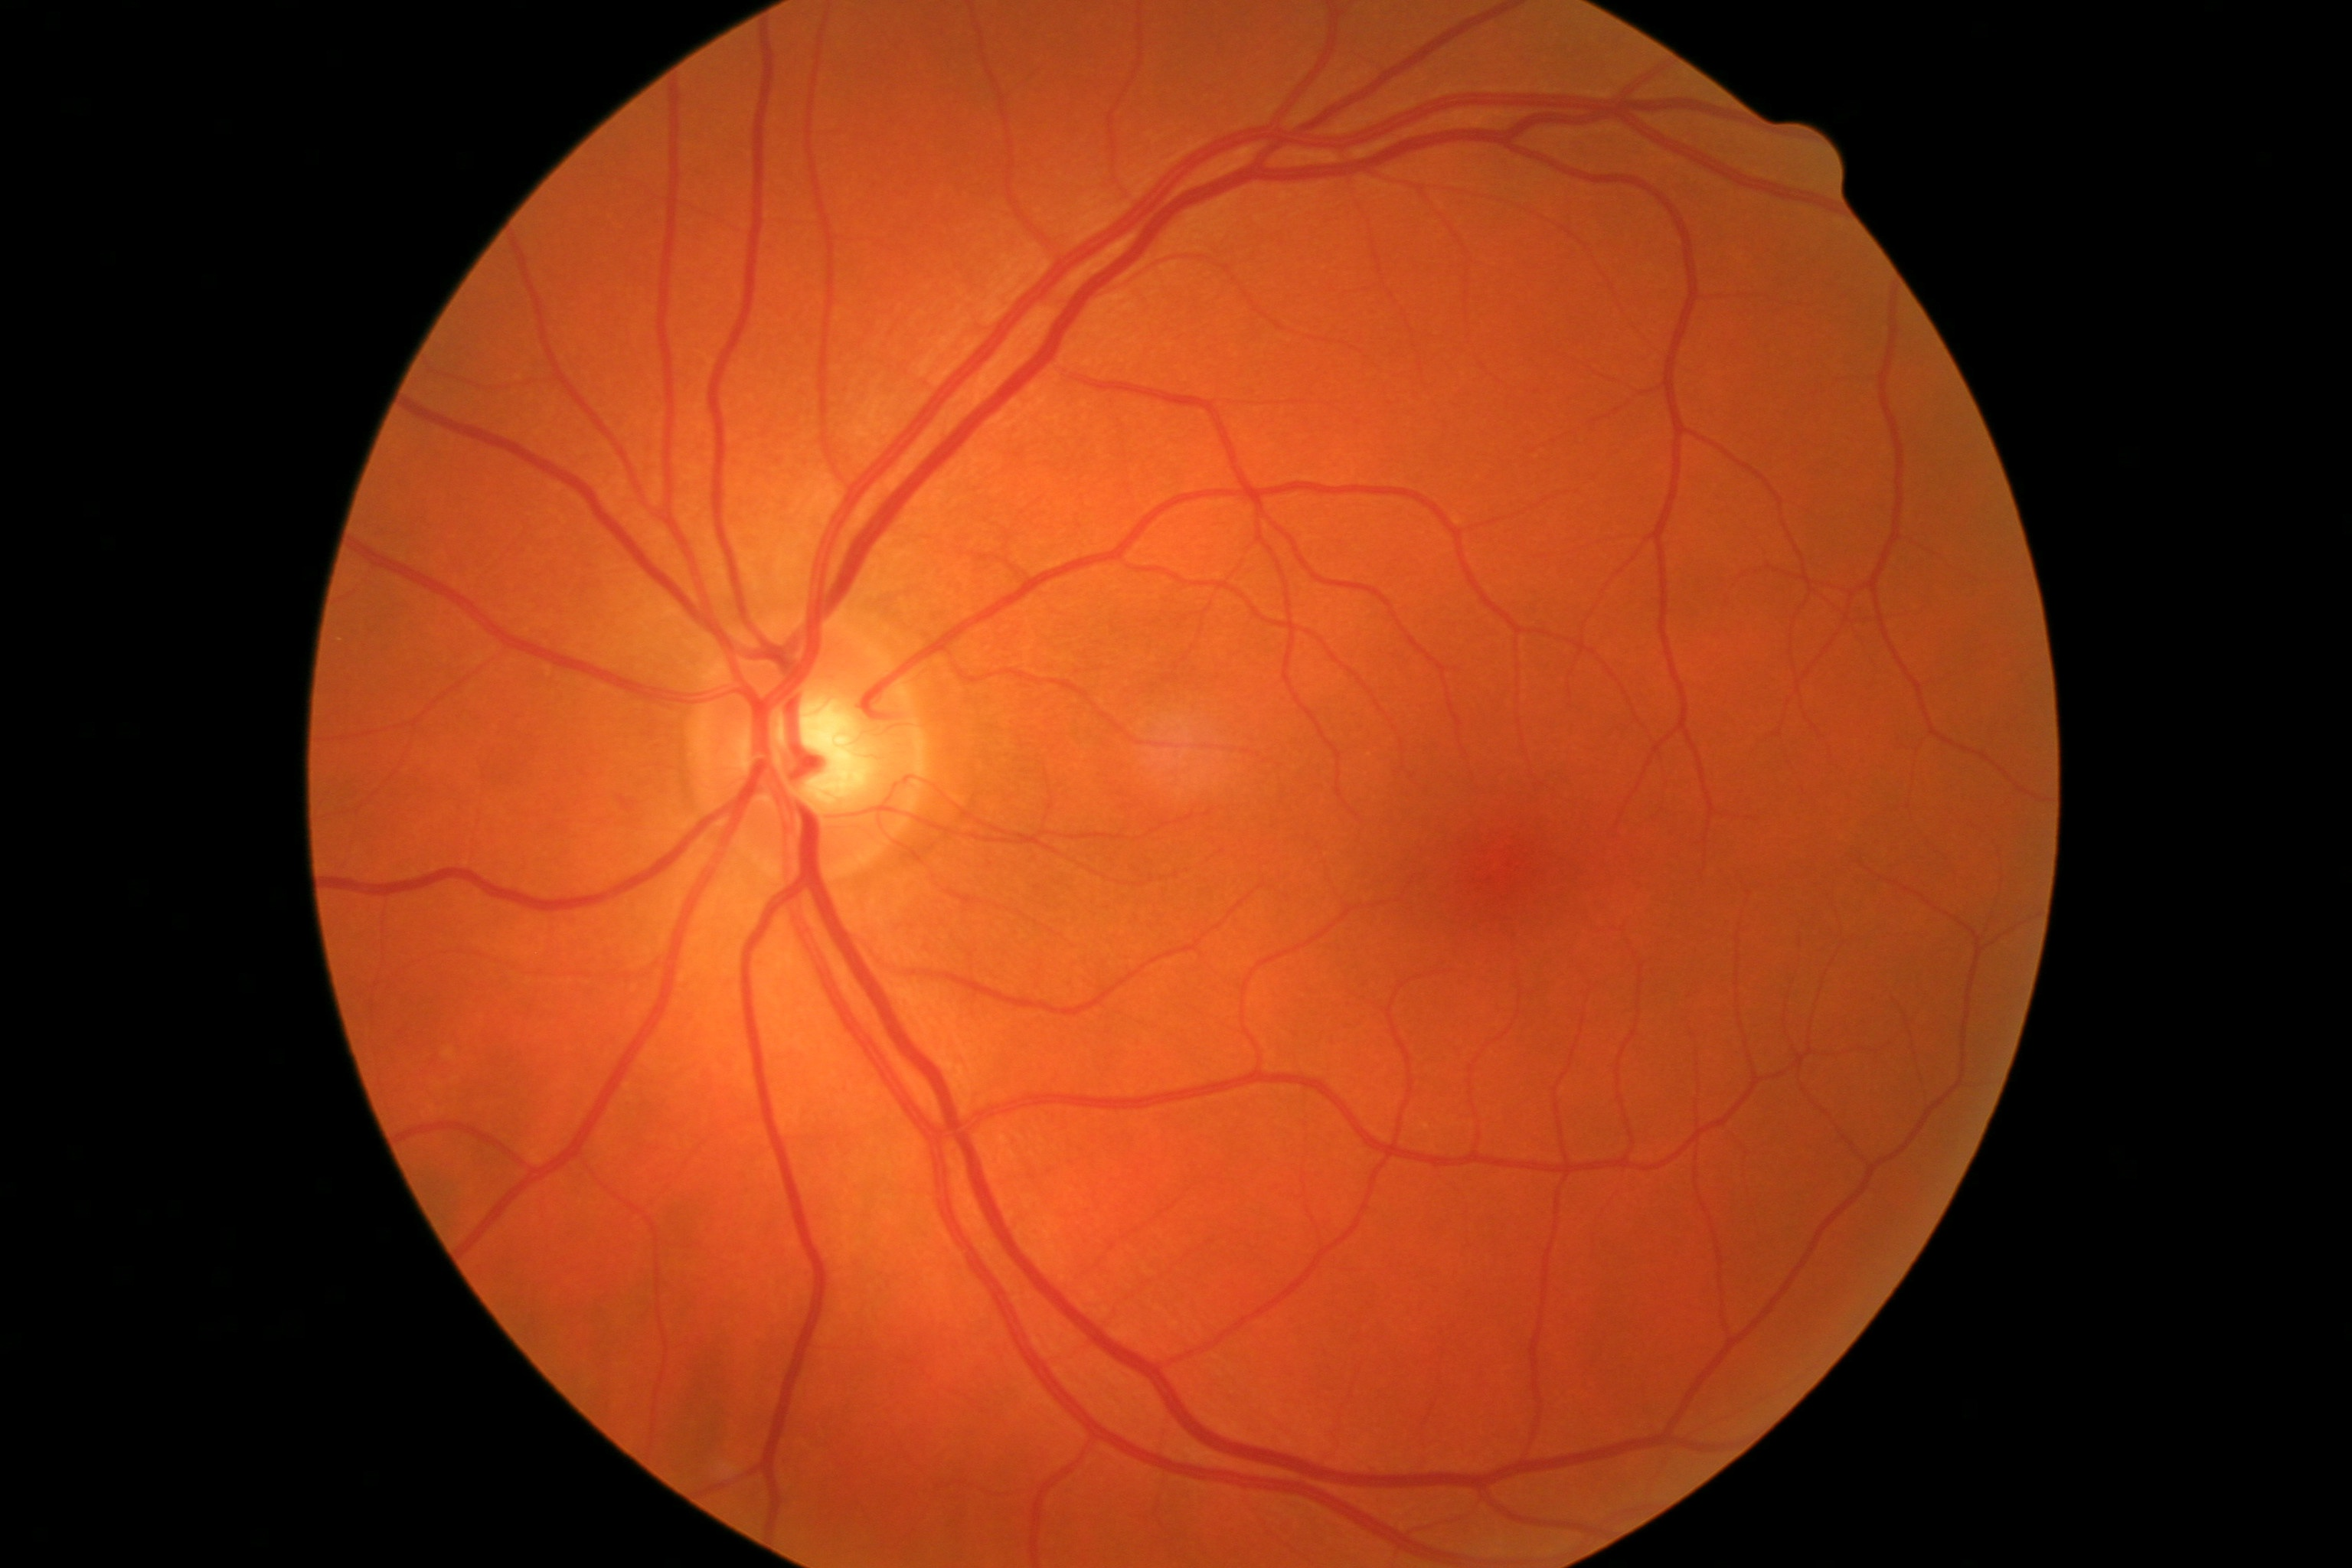
\includegraphics[height=1.3in,width=1.6in]{./images/10031_left.jpeg}}
	\subfigure[Label 1]{\label{fig:a}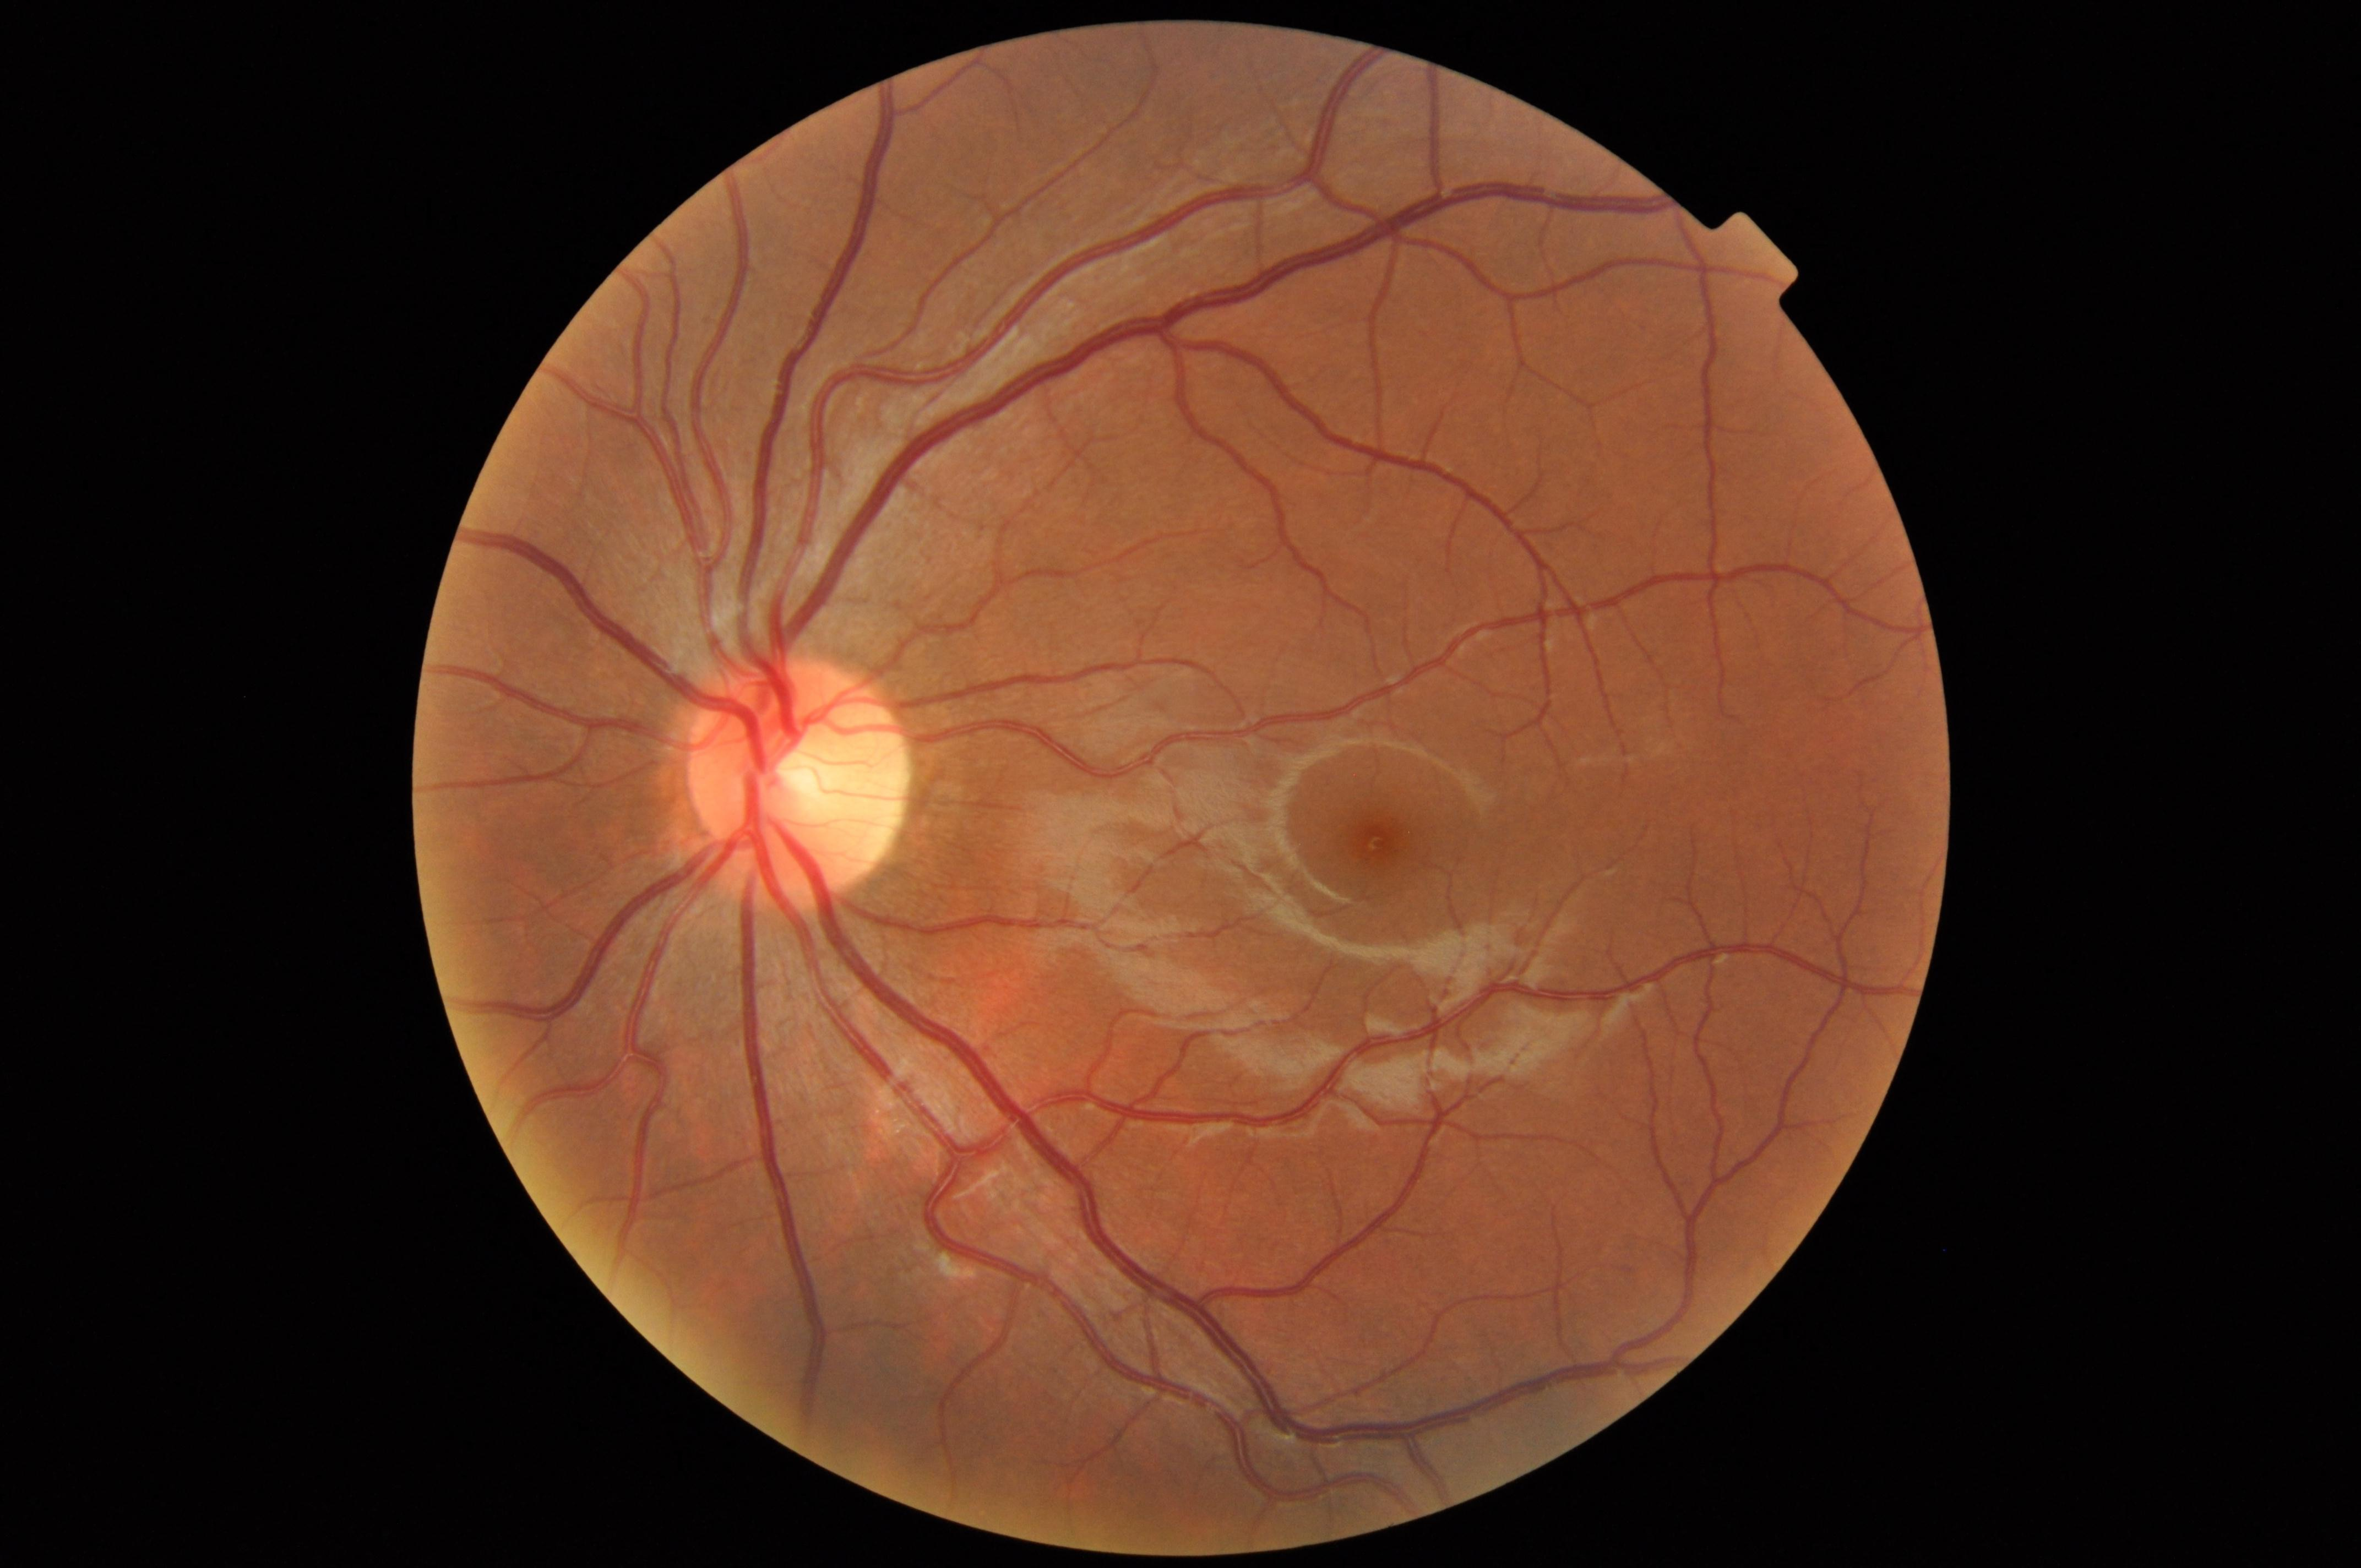
\includegraphics[height=1.3in,width=1.6in]{./images/10727_left.jpeg}}
	\subfigure[Label 2]{\label{fig:a}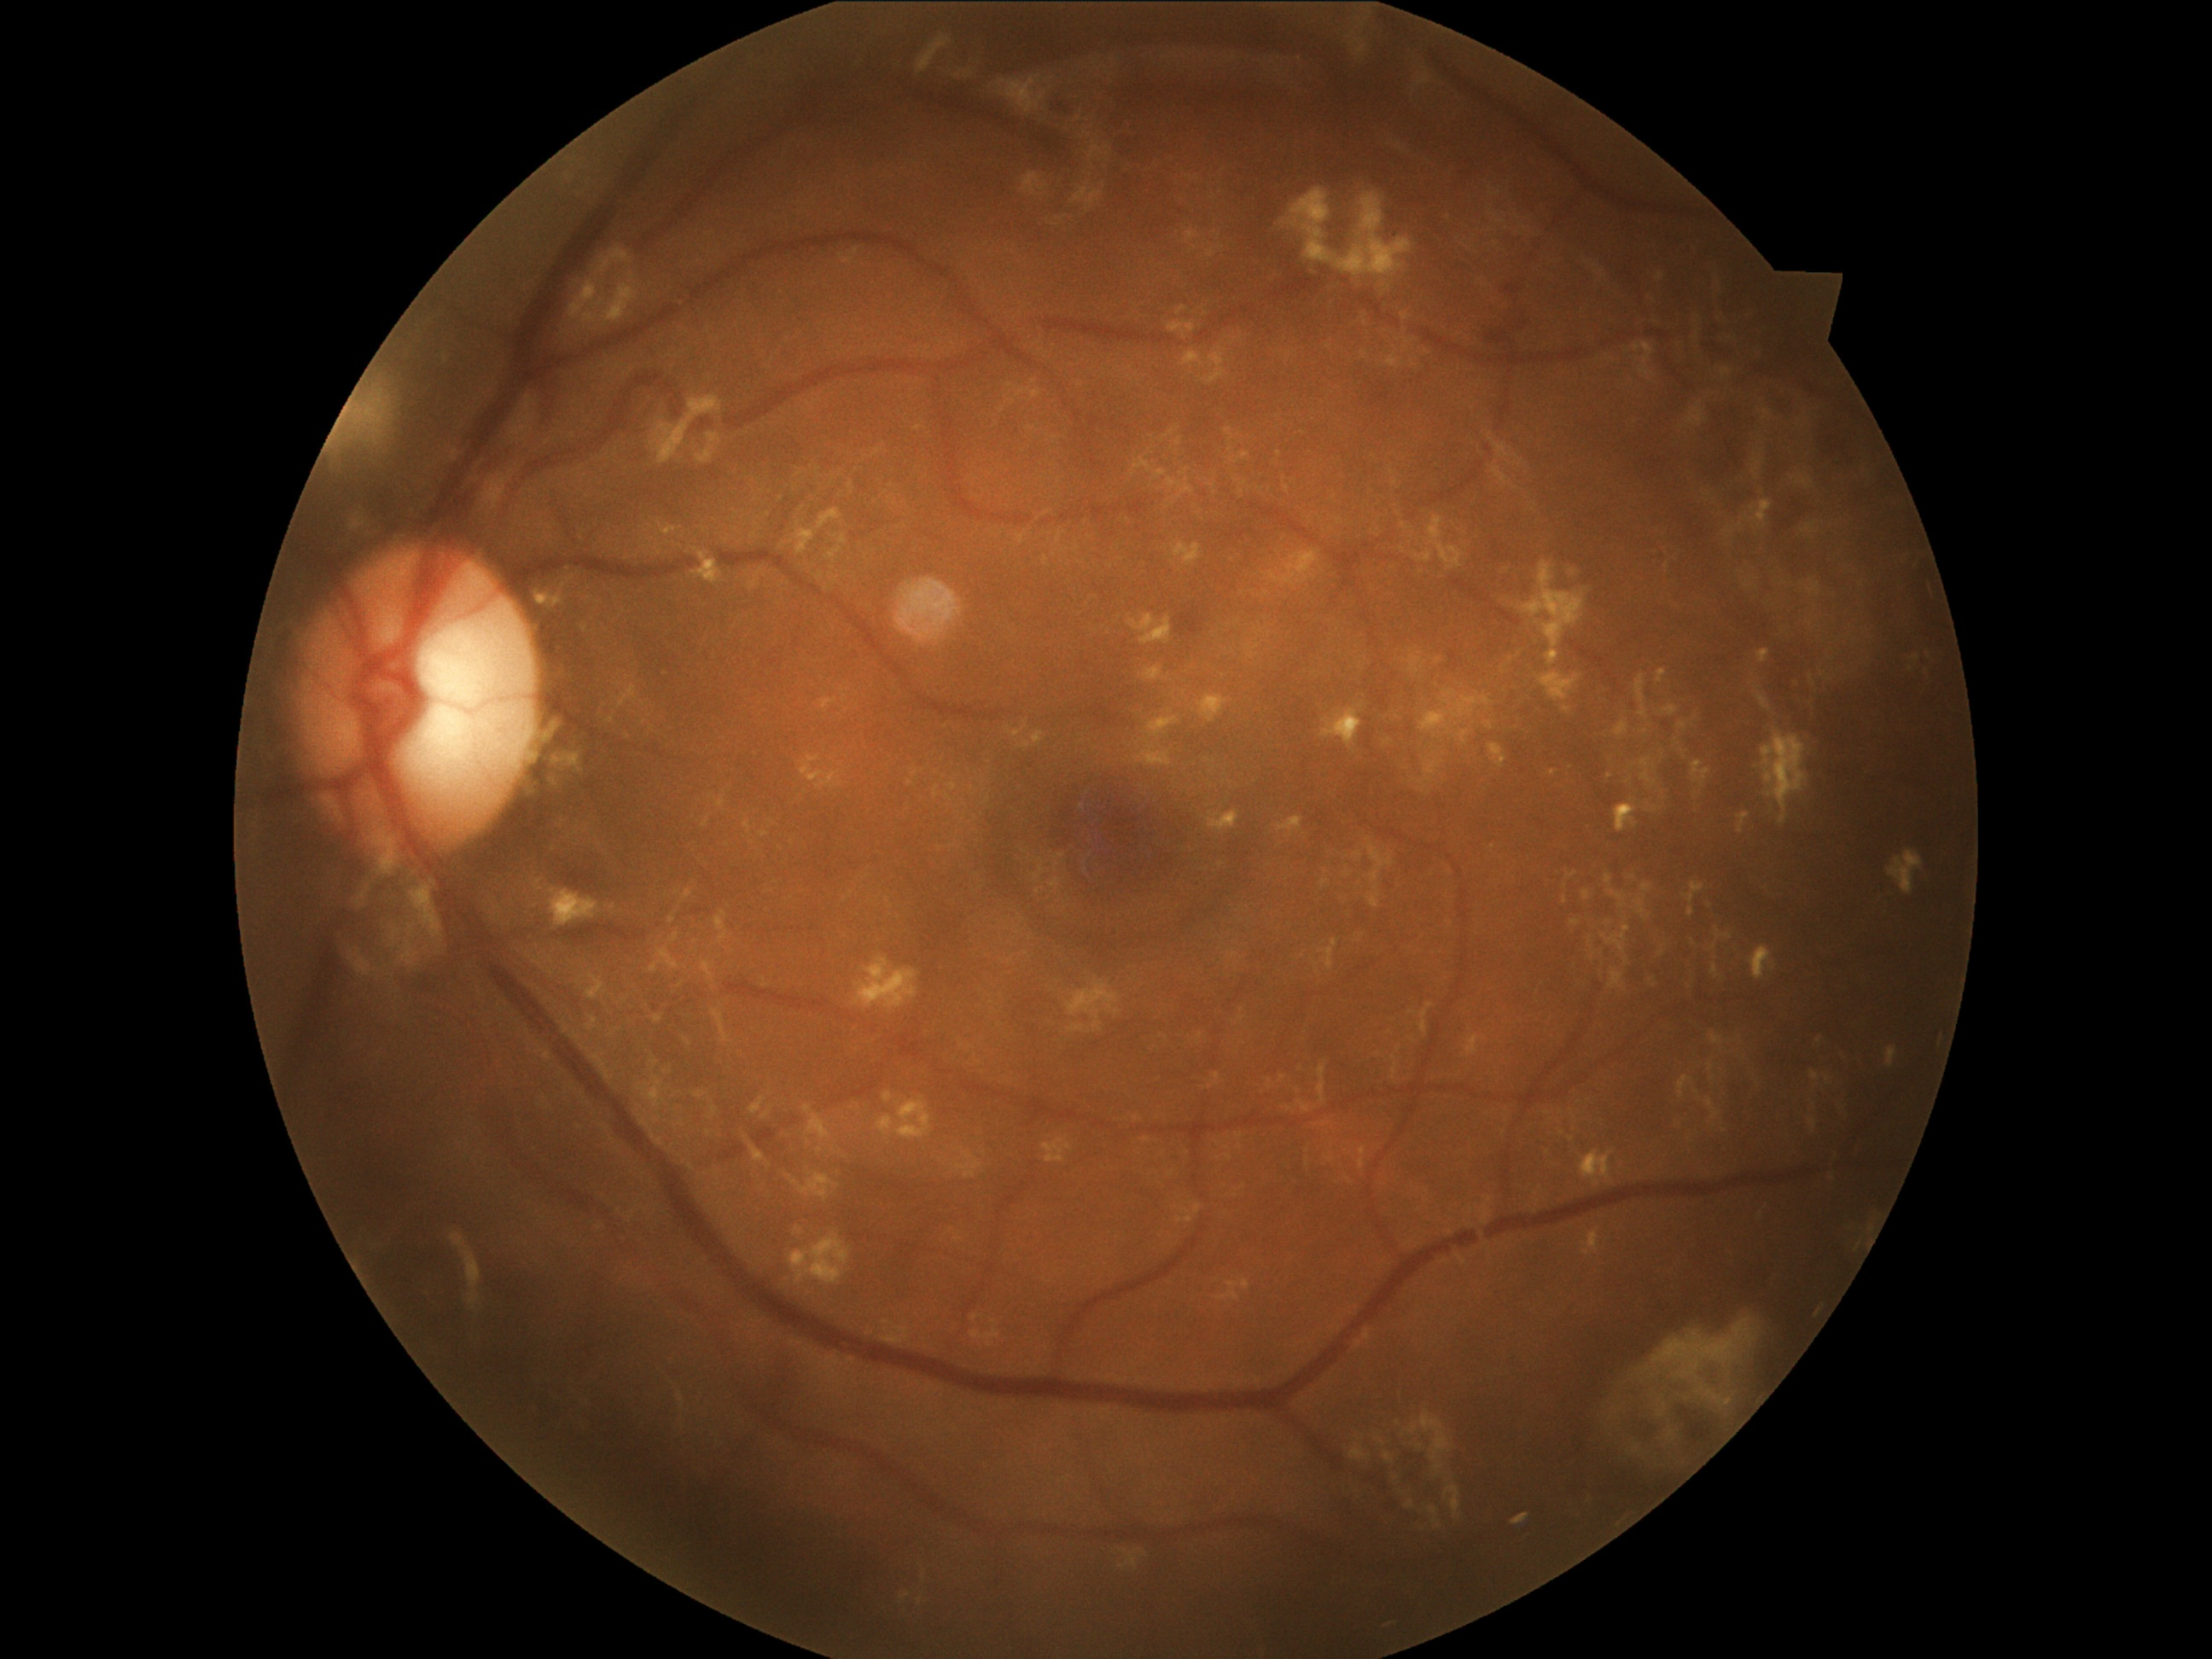
\includegraphics[height=1.3in,width=1.6in]{./images/15138_left.jpeg}}
\end{figure}  
\begin{figure}[H]
	\centering
	\subfigure[Label 3]{\label{fig:a}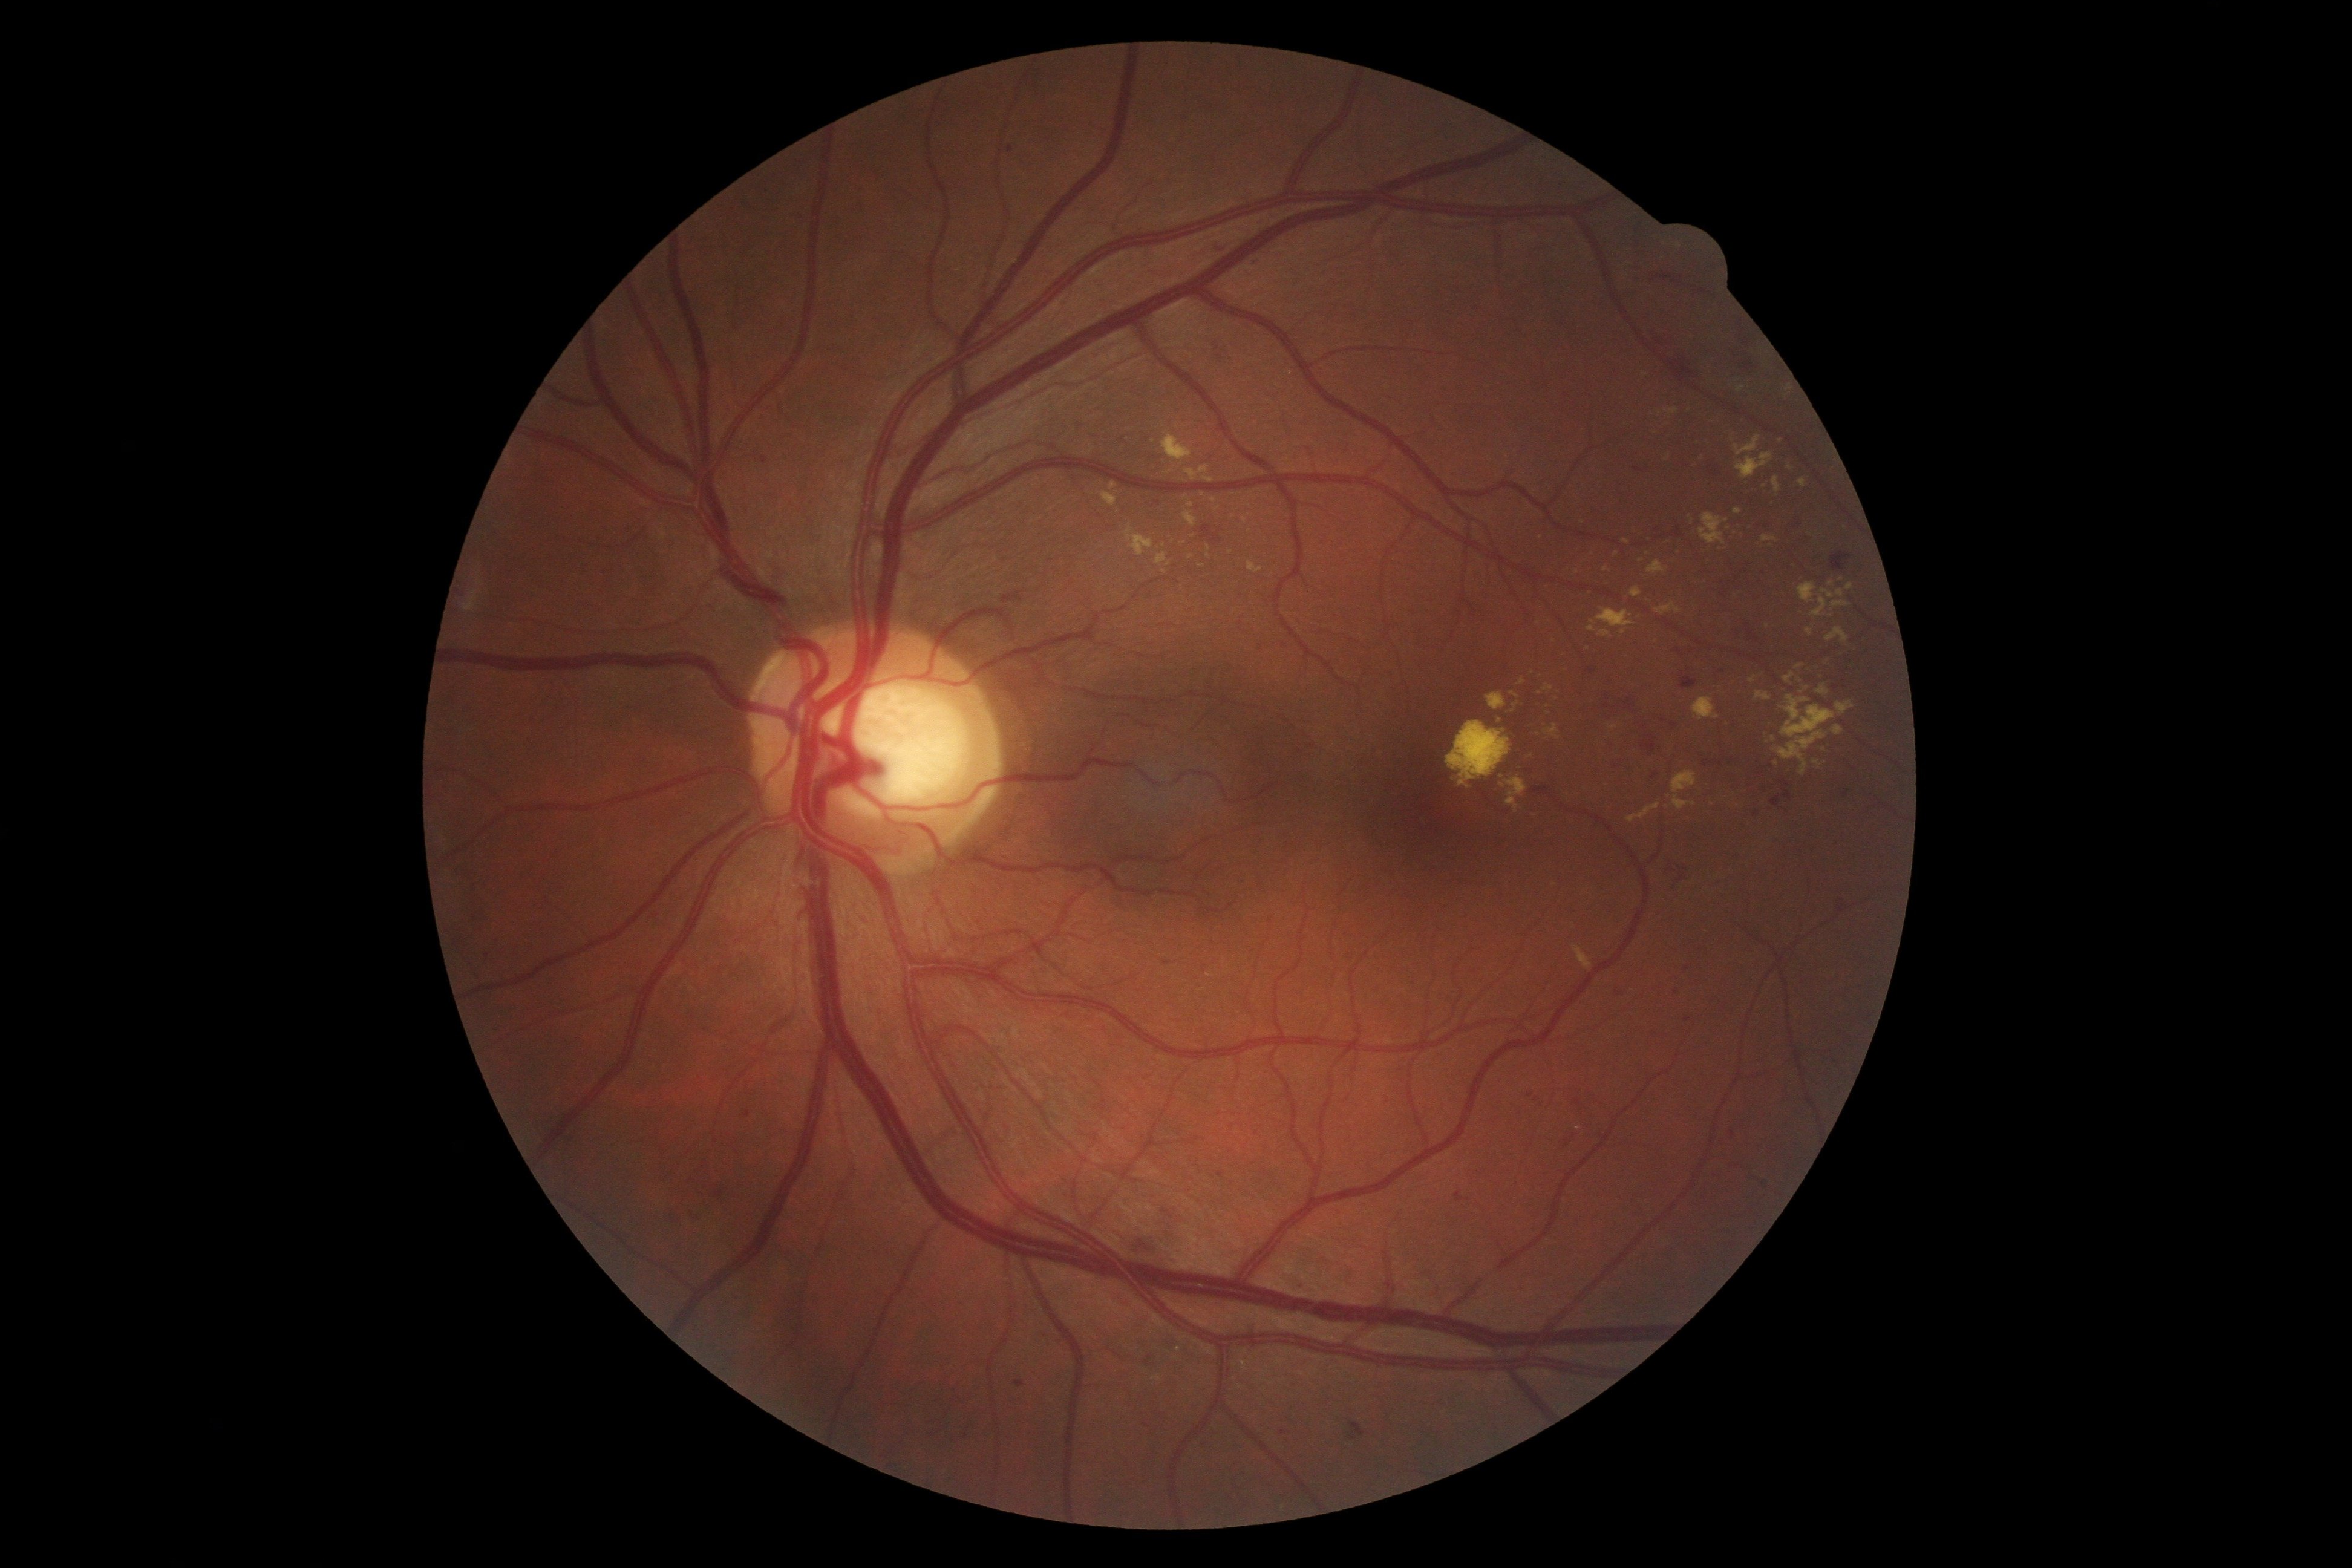
\includegraphics[height=1.3in,width=1.6in]{./images/19367_left.jpeg}}
	\subfigure[Label 4]{\label{fig:a}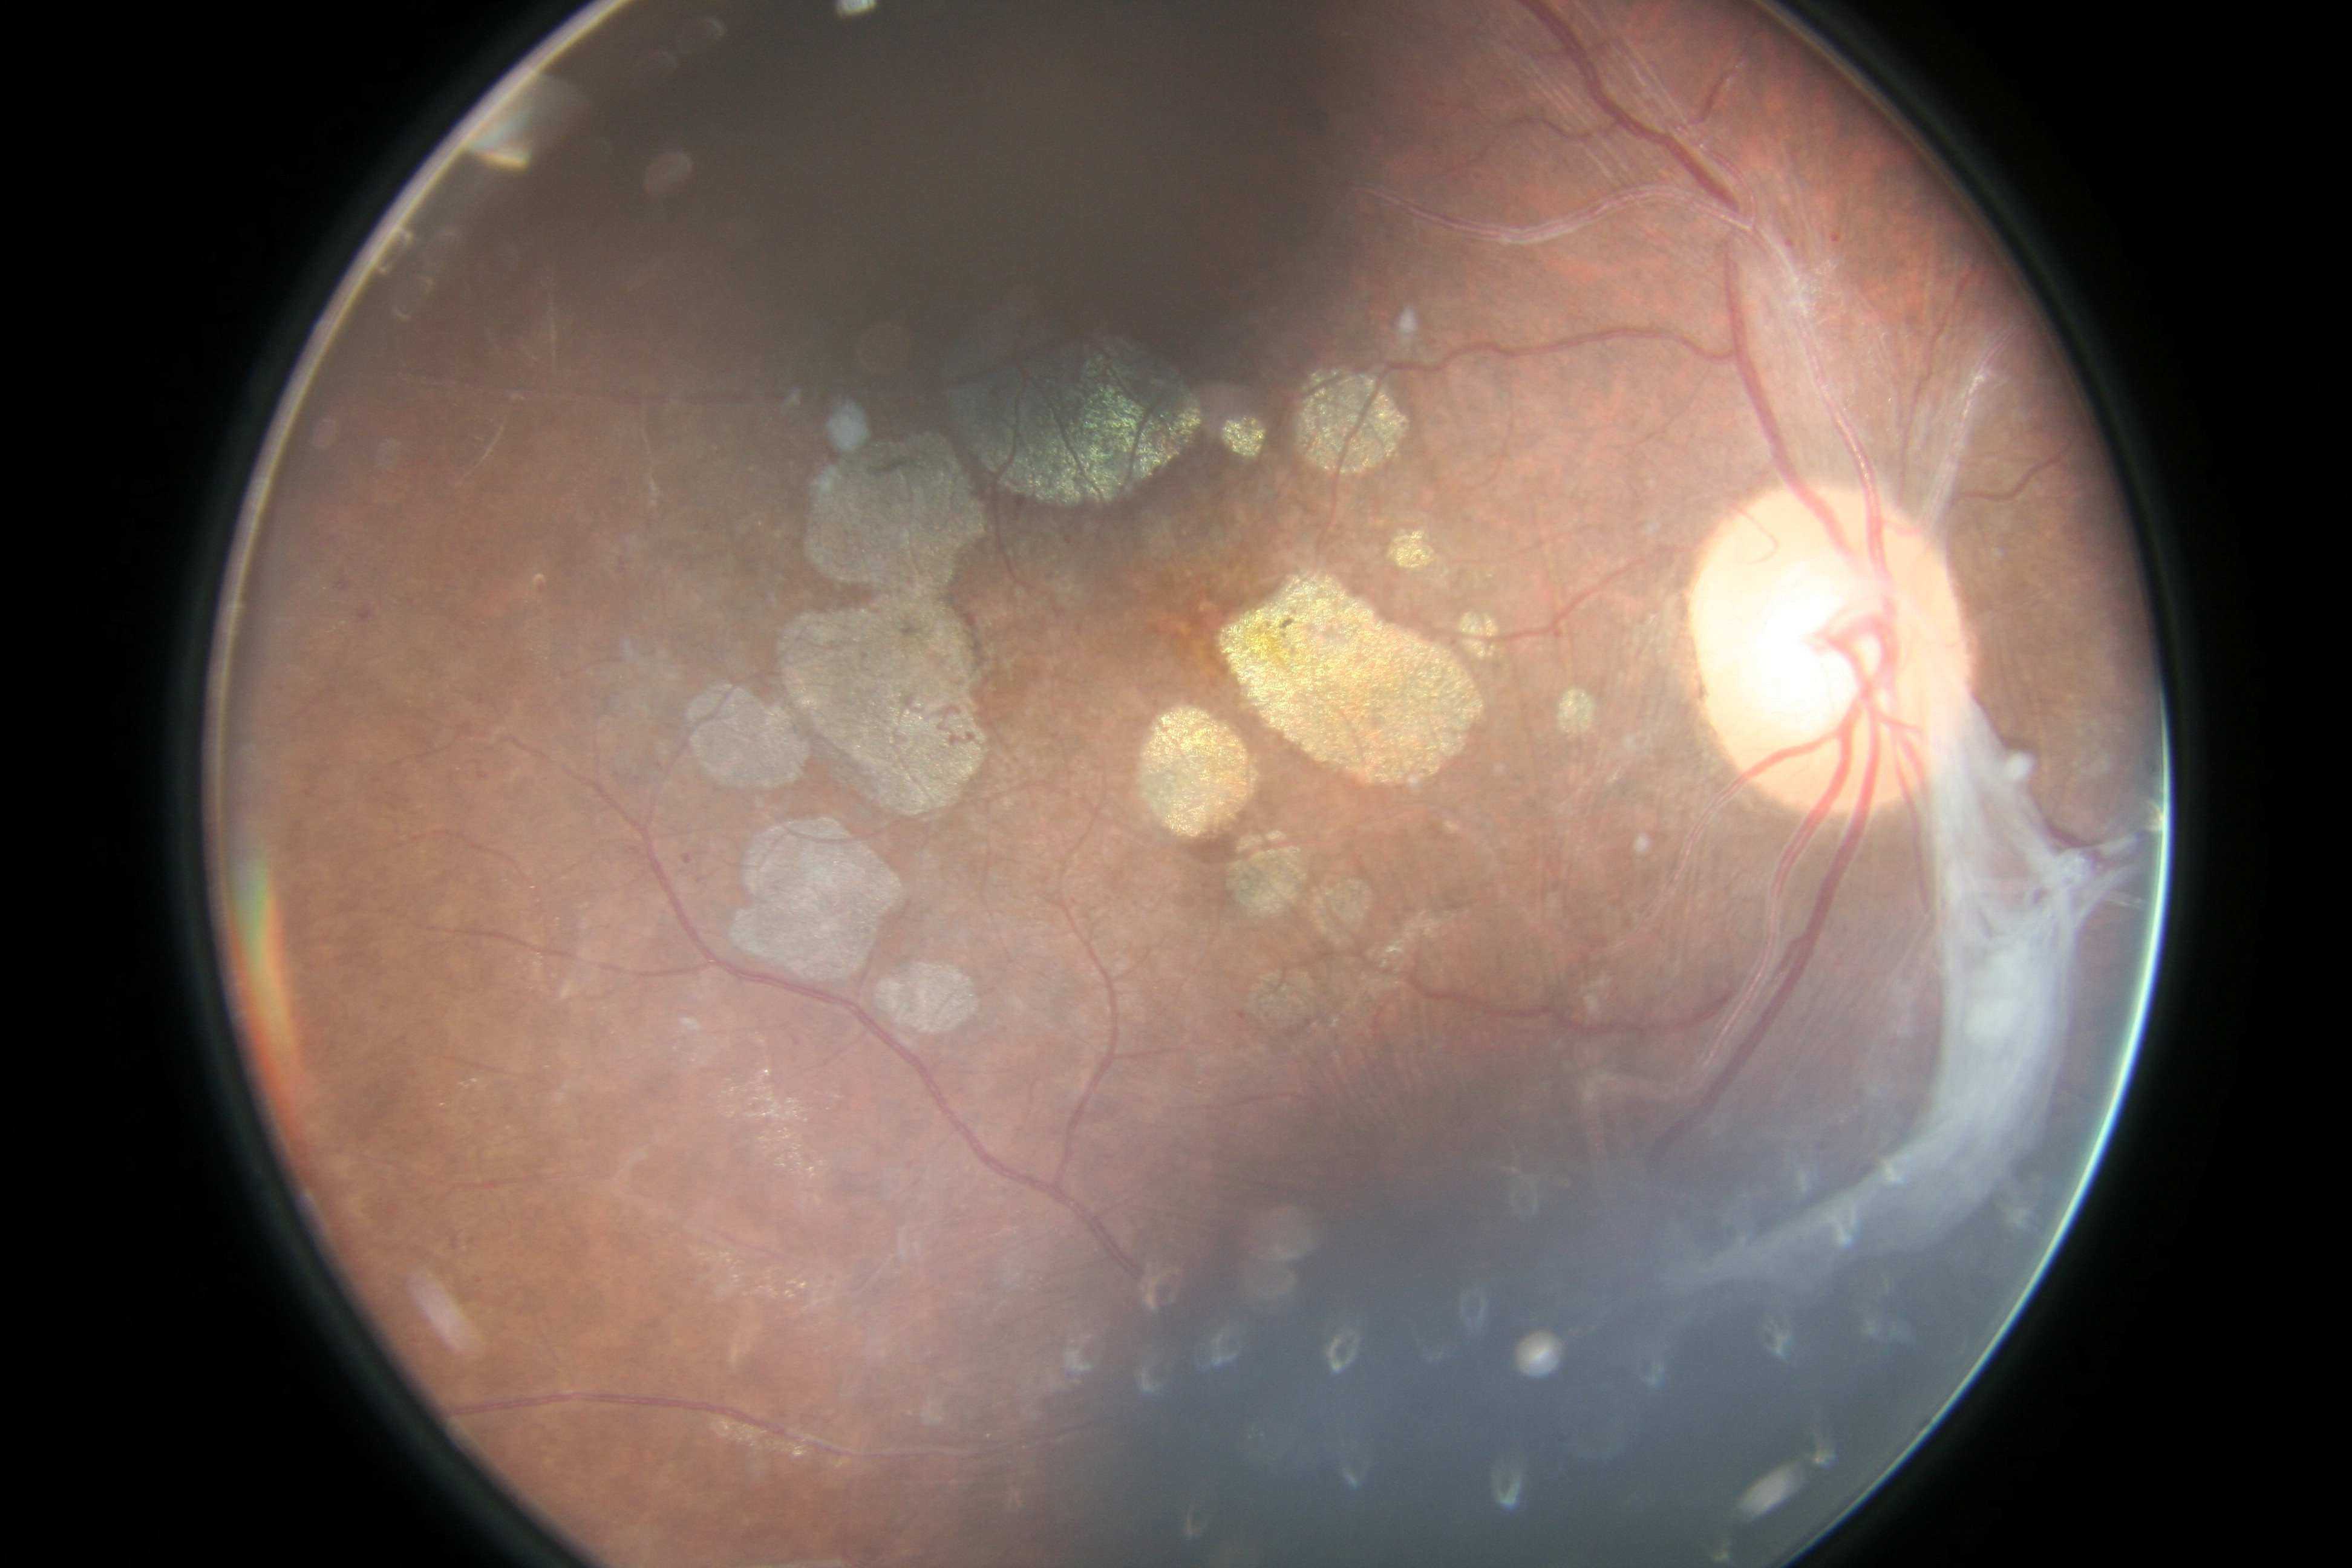
\includegraphics[height=1.3in,width=1.6in]{./images/1084_left.jpeg}}
\end{figure} 
For ideas about some domain-dependent features, we referred to a paper titled ``Screening for Diabetic Retinopathy Using Computer Vision and Physiological Markers'' \cite{hann2009} which was written by Christoper E. Hann and colleagues. In this paper, Hann describes methods of detecting exudates, which are defined as leakages of lipids from vessels in the eye, and dot hemorrhages, which are small ruptures in the deep layers of the retina; both of these conditions aid in characterizing the severity of the disease. \\ \\
However, an important point to note regarding Hann's work is that he does not categorize images into classes using exudate and hemorrhage features. Instead, he evaluates his identification methods by computing Positive Predictive Value (PPV) and Negative Predictive Value (NPV) scores where a human manually counts the number of exudate regions and dot hemorrhages and these values are compared with the output of the identification algorithm. The PPV and NPV results were very good for both exudate (PPV: 97\%, NPV: 95\%) and hemorrhage (PPV: 96\%, NPV: 100\%) identification tasks. \\ \\
In our work, we utilize these identification methods in a different way to build a multiclass classifier. We also attempt to perform classification using generalized approaches such as color histograms and SIFT feature vectors.

\section{Generalized Approaches}

\subsection{Color Histograms}

We first attempt to classify images using color histograms. For each image, we compute 16 bin histograms for each patch in our 3-level spatial pyramid. We have 1 histogram for the first level, 4 for the second, and 16 for the third giving us 21 total histograms. We concatenate these histograms into a single $(21 \times 16) \times 1$ feature vector for the image. We then experiment with both histogram intersection and nearest-neighbor Euclidean distance scoring schemes. We use 10 fold cross validation in evaluation. Our results are below.

\begin{tabular}{| l | l | l |}
\hline
Eye side & Grading Scheme & Average accuracy across 10 folds \\ \hline
Left & Histogram Intersection & 17.2\% \\ \hline
Left & Nearest-Neighbor & 22.8\% \\ \hline
Right & Histogram Intersection & 18.6\% \\ \hline
Right & Nearest-Neighbor & 21.7\% \\ \hline
\end{tabular} 

We observe that color histograms do not yield good results. We suspect that because the color variance is large and each class does not have a distinctive color to aid in classification, the performance is consequently poor. The color variance is affected by the different lighting schemes in each image as well as the varying natural eye colors. Below we show images that are all labeled 0, but have drastically different lighting and colors.

\newpage

\begin{figure*}[!htp]
  \centering
  \subfigure{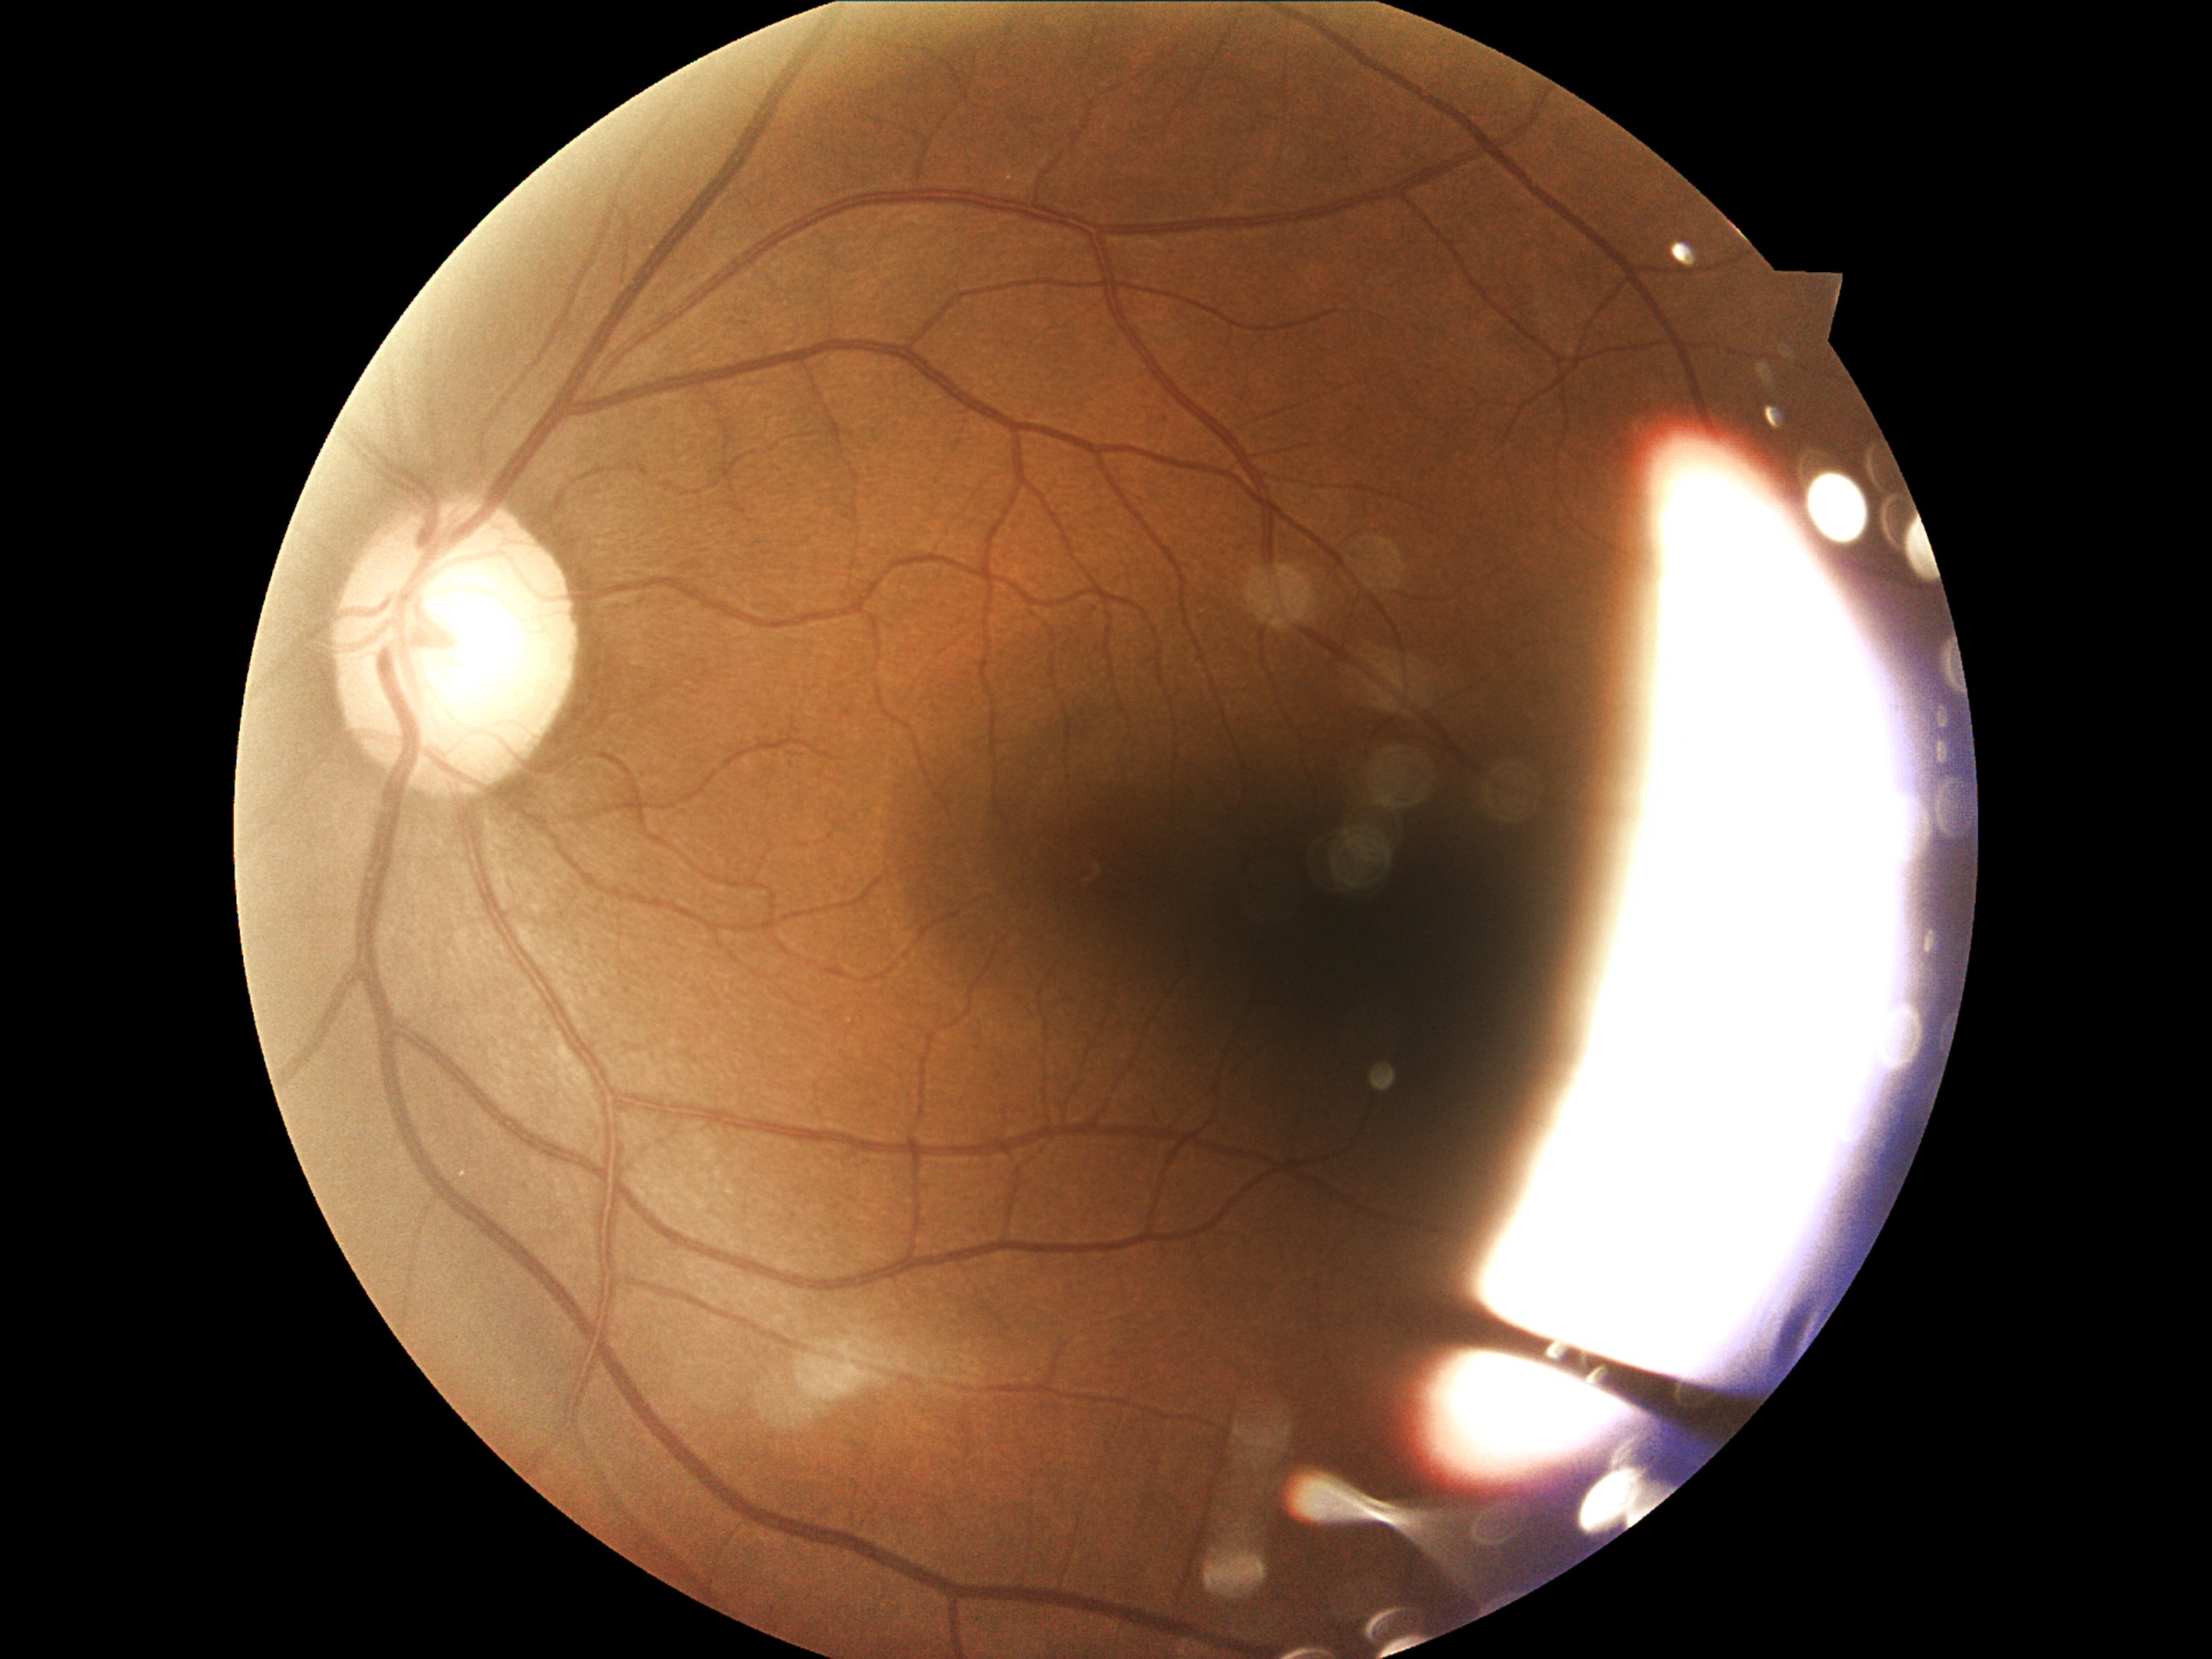
\includegraphics[height=1.3in,width=1.6in]{./images/Color_Histogram/318_left.jpeg}
}
  \subfigure{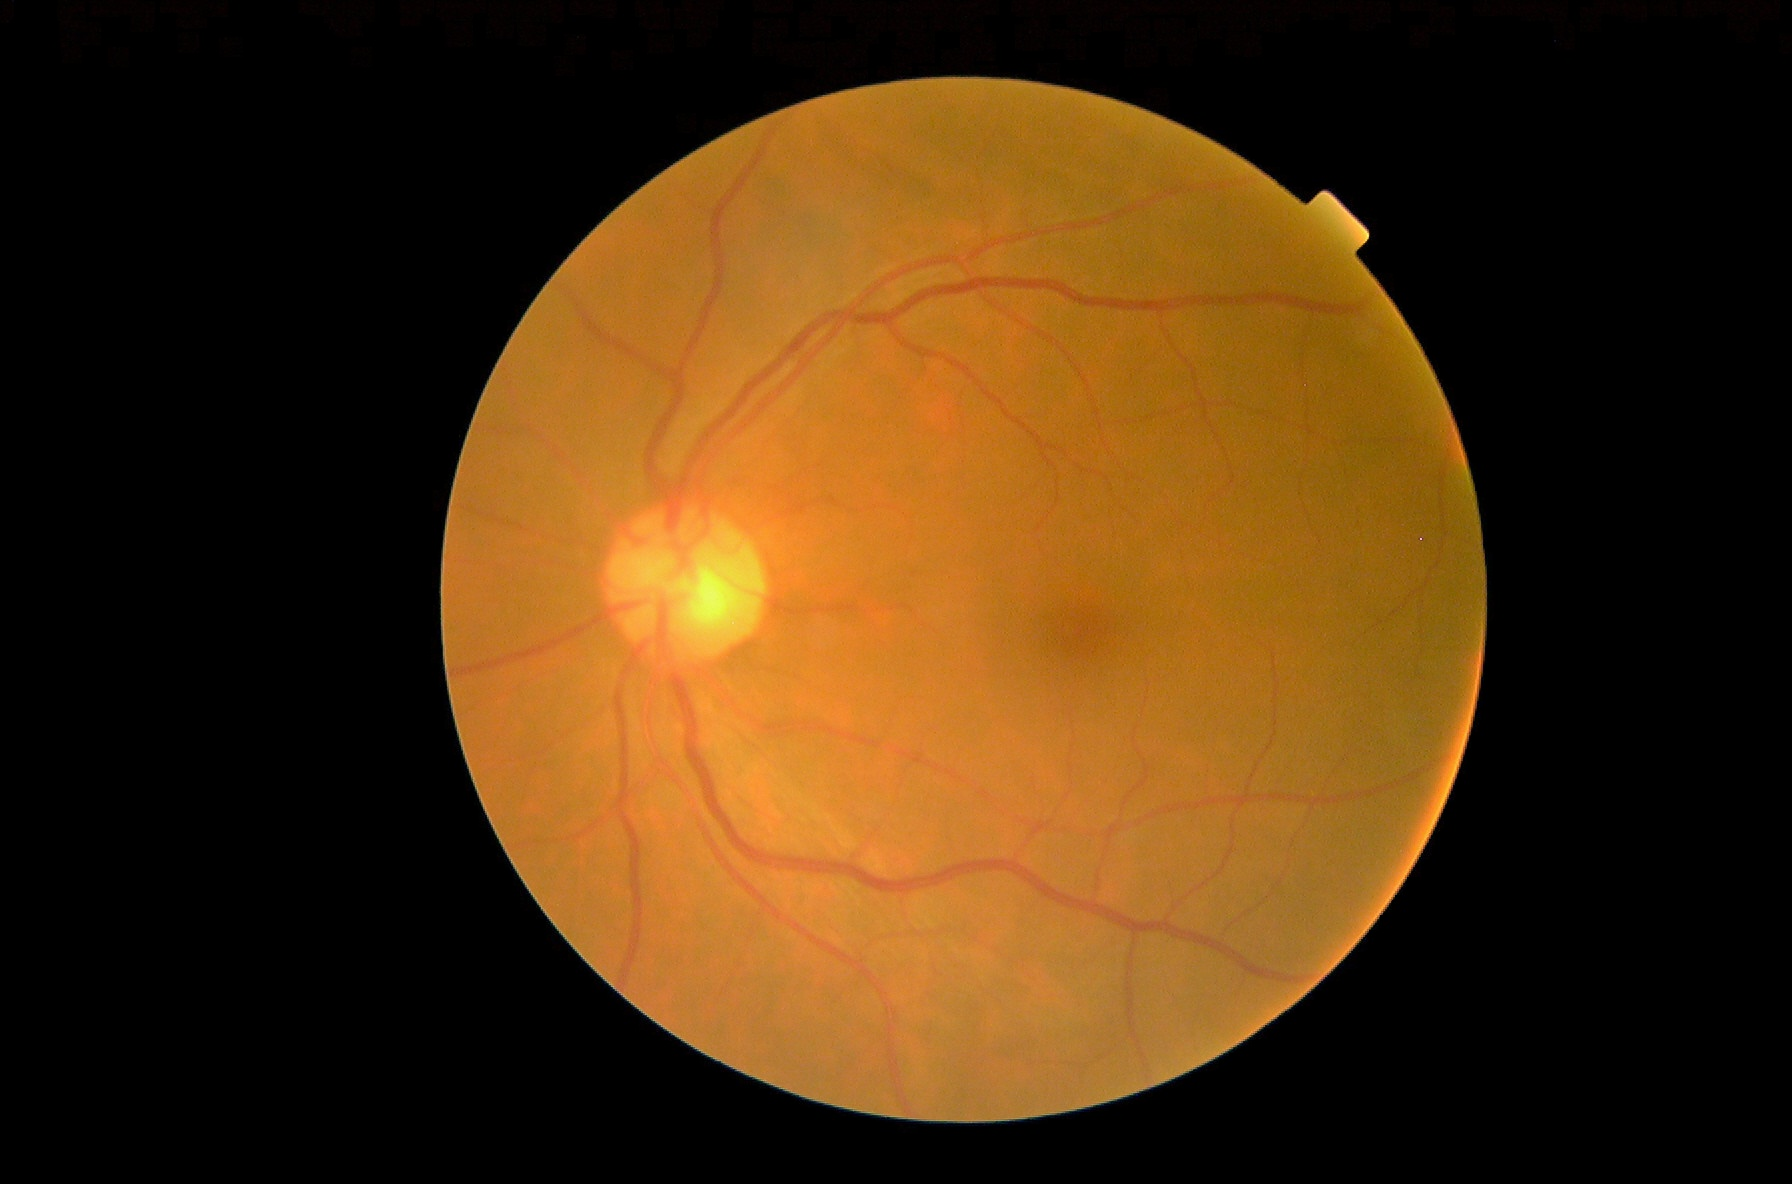
\includegraphics[height=1.3in,width=1.6in]{./images/Color_Histogram/72_left.jpeg}
  }
  \subfigure{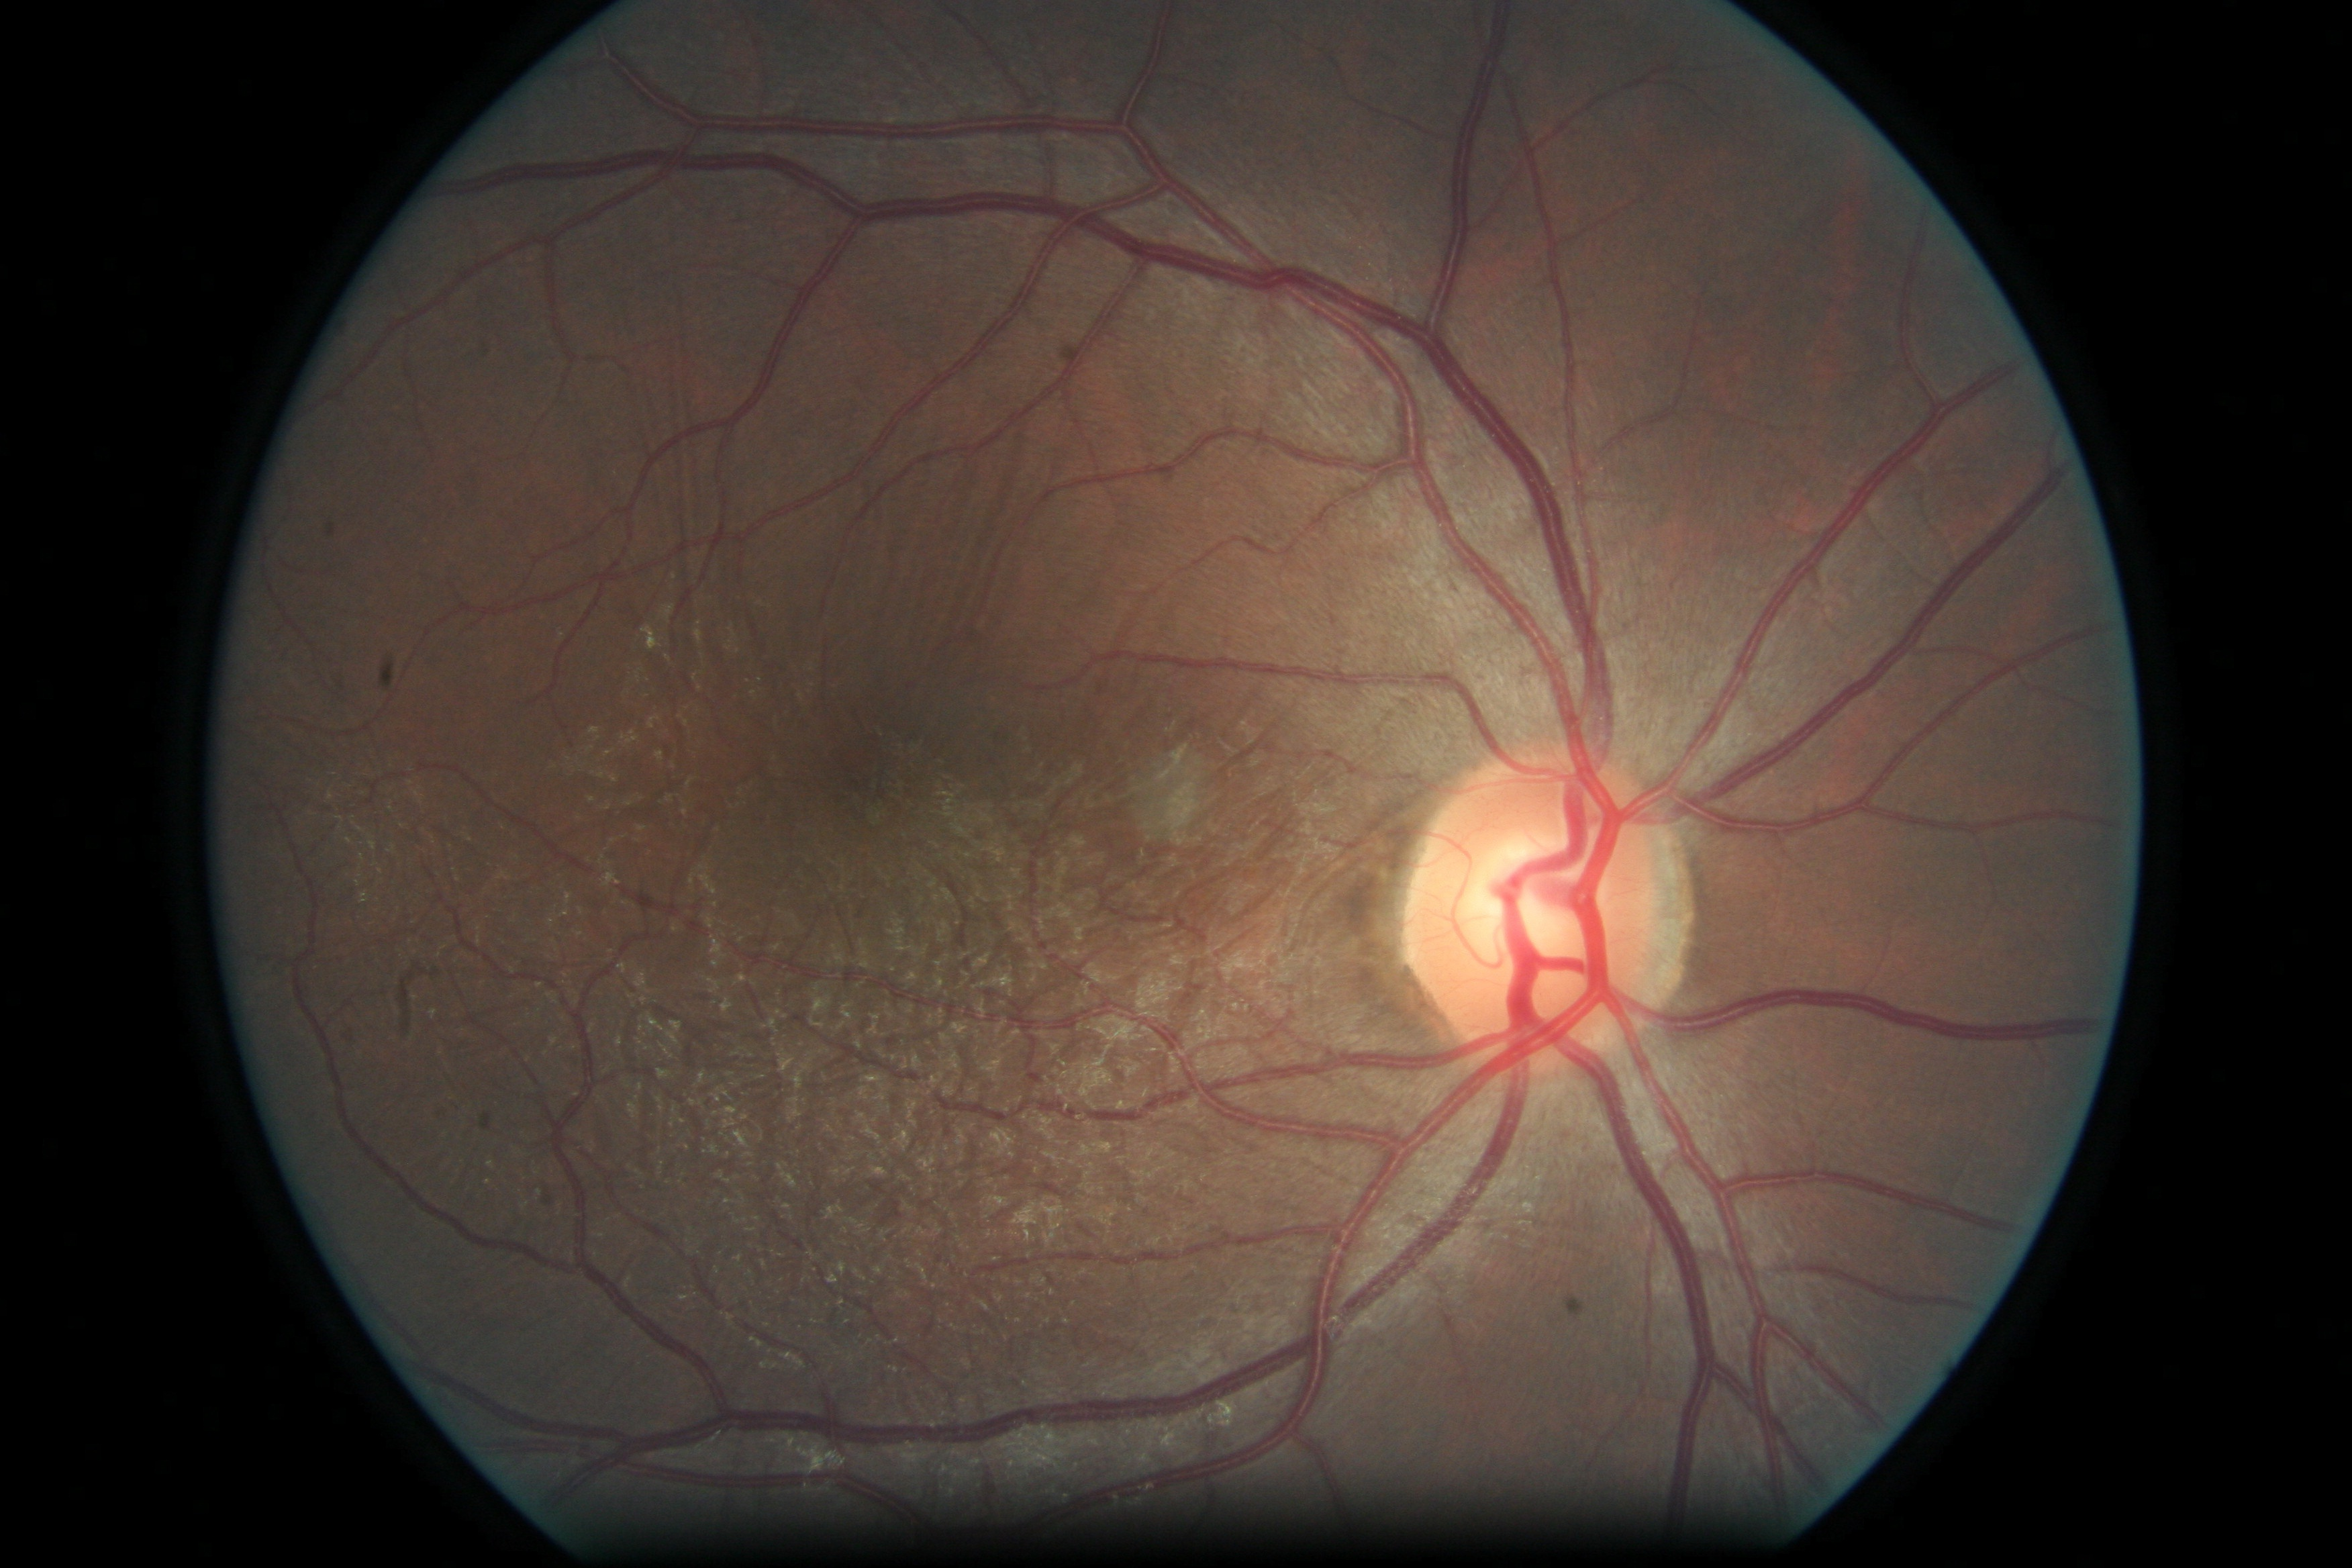
\includegraphics[height=1.3in,width=1.6in]{./images/Color_Histogram/73_left.jpeg}
  }
  \subfigure{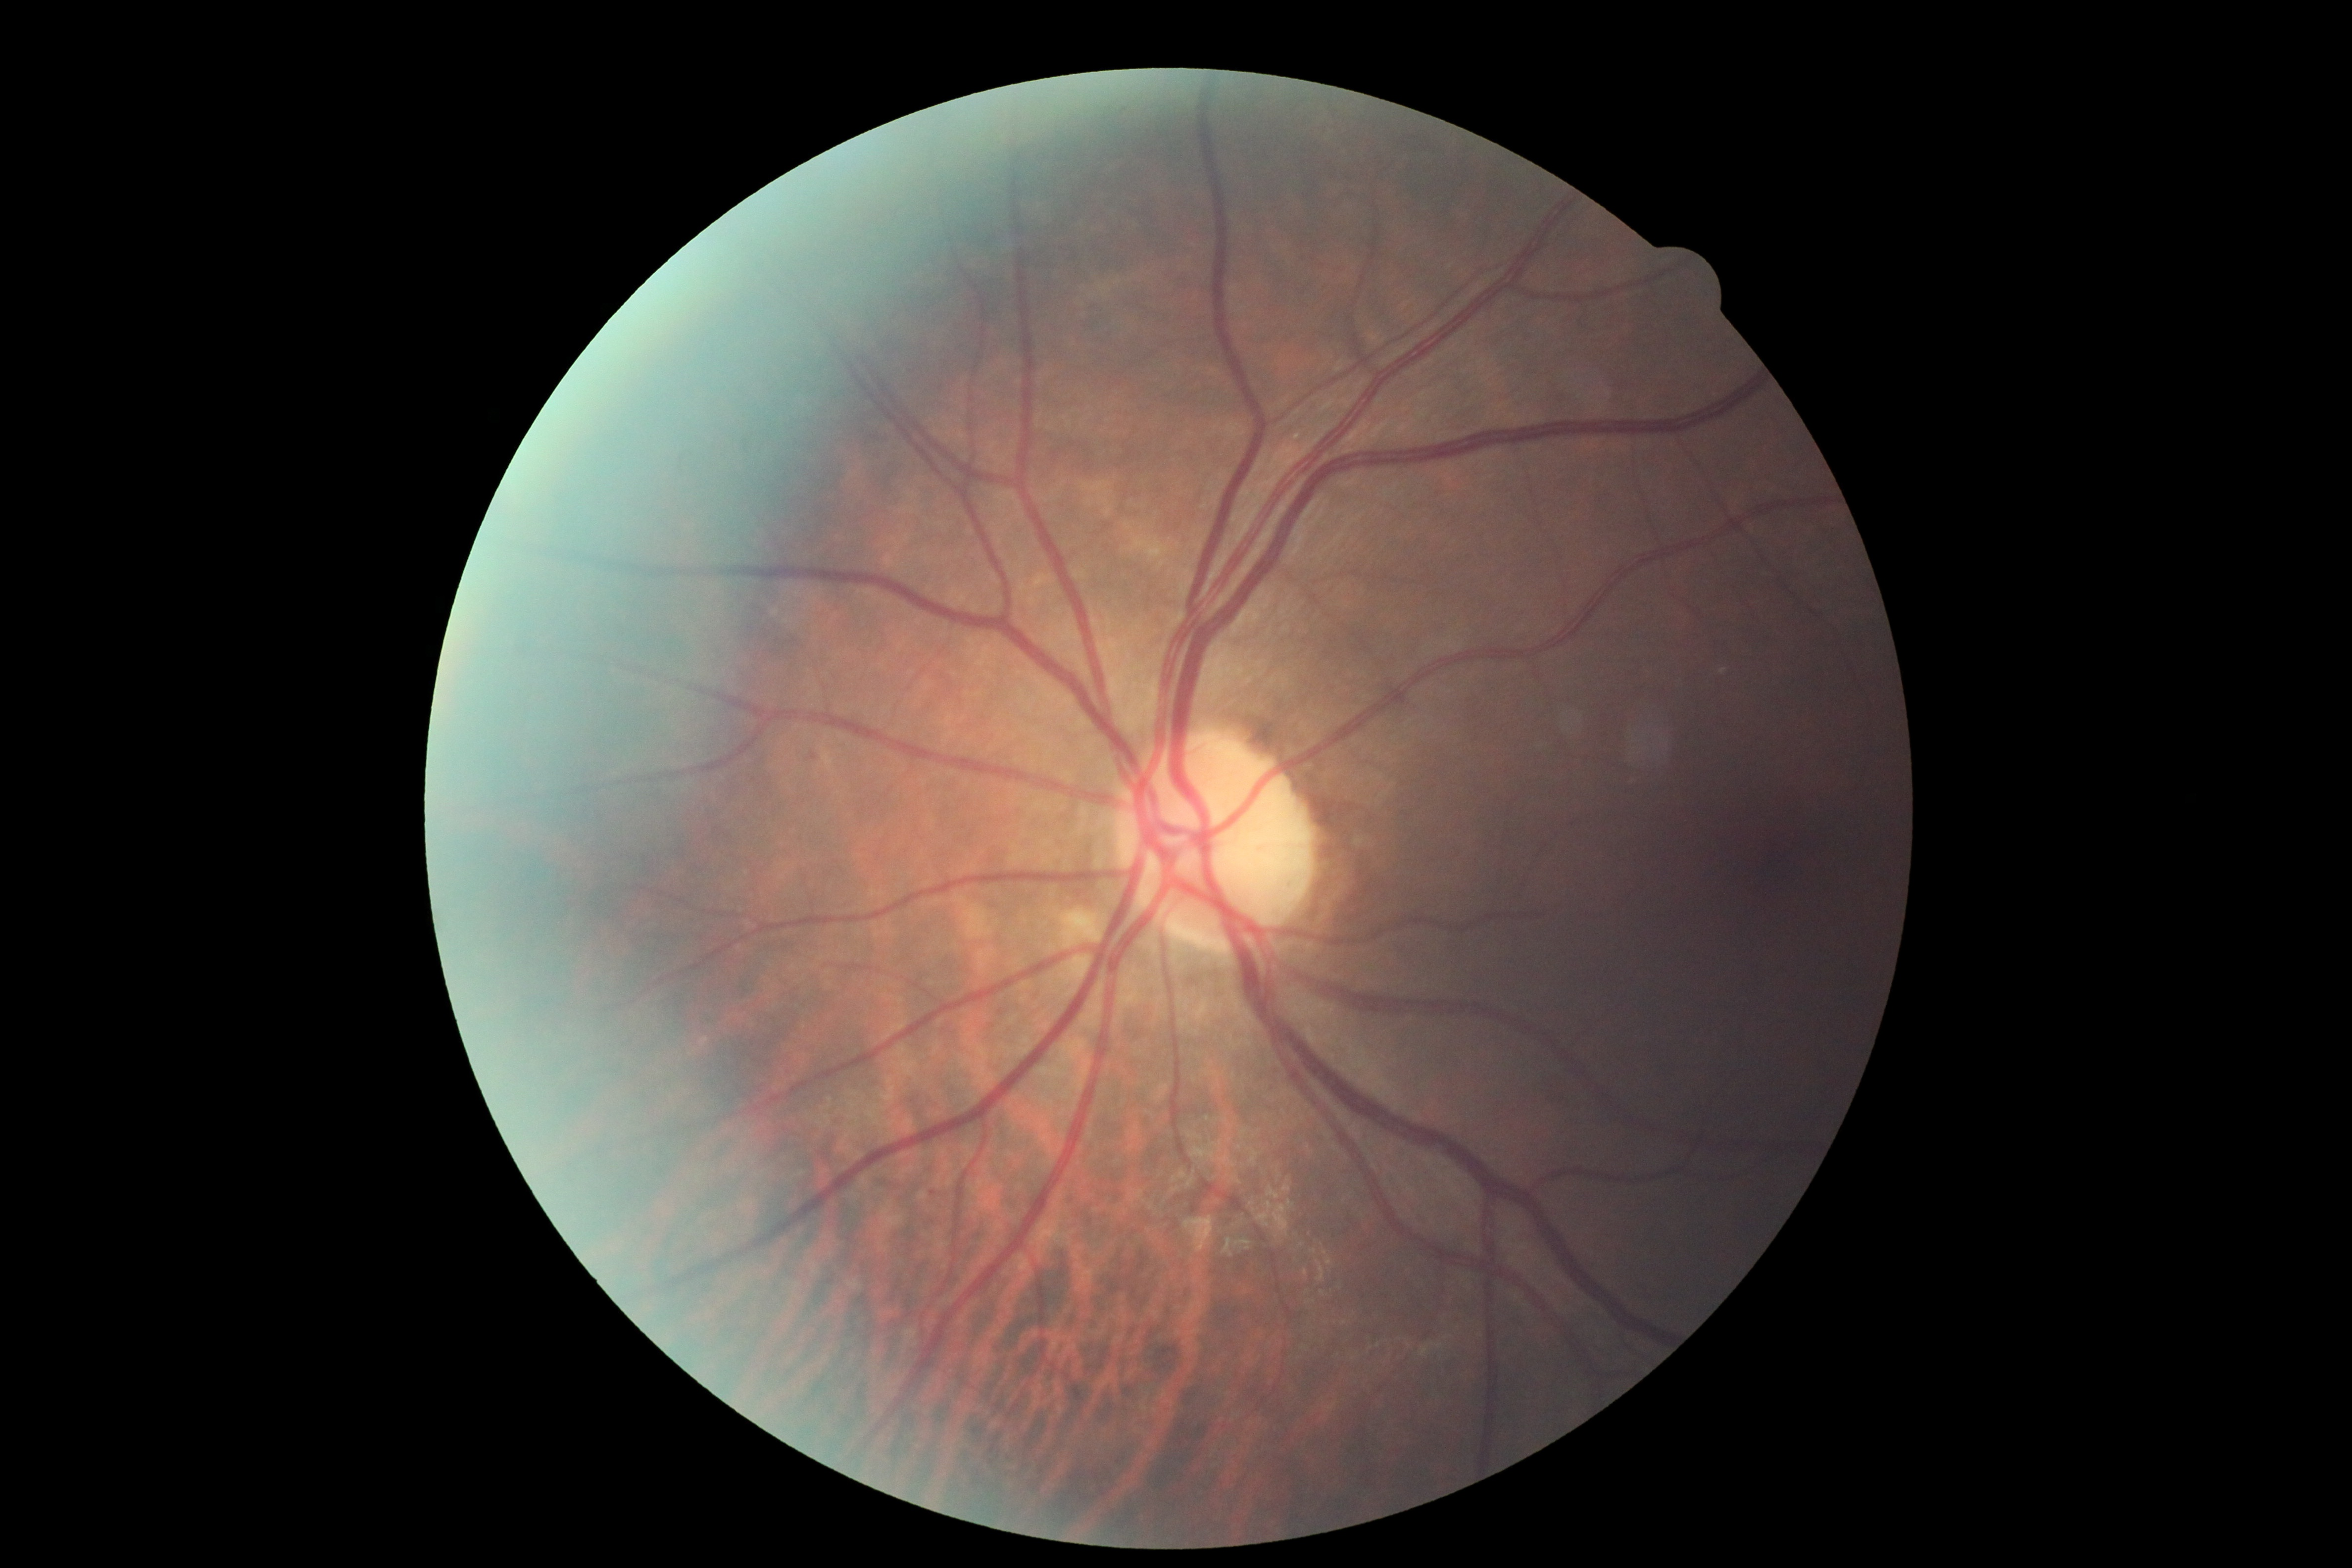
\includegraphics[height=1.3in,width=1.6in]{./images/Color_Histogram/10_left.jpeg}
  }
  \subfigure{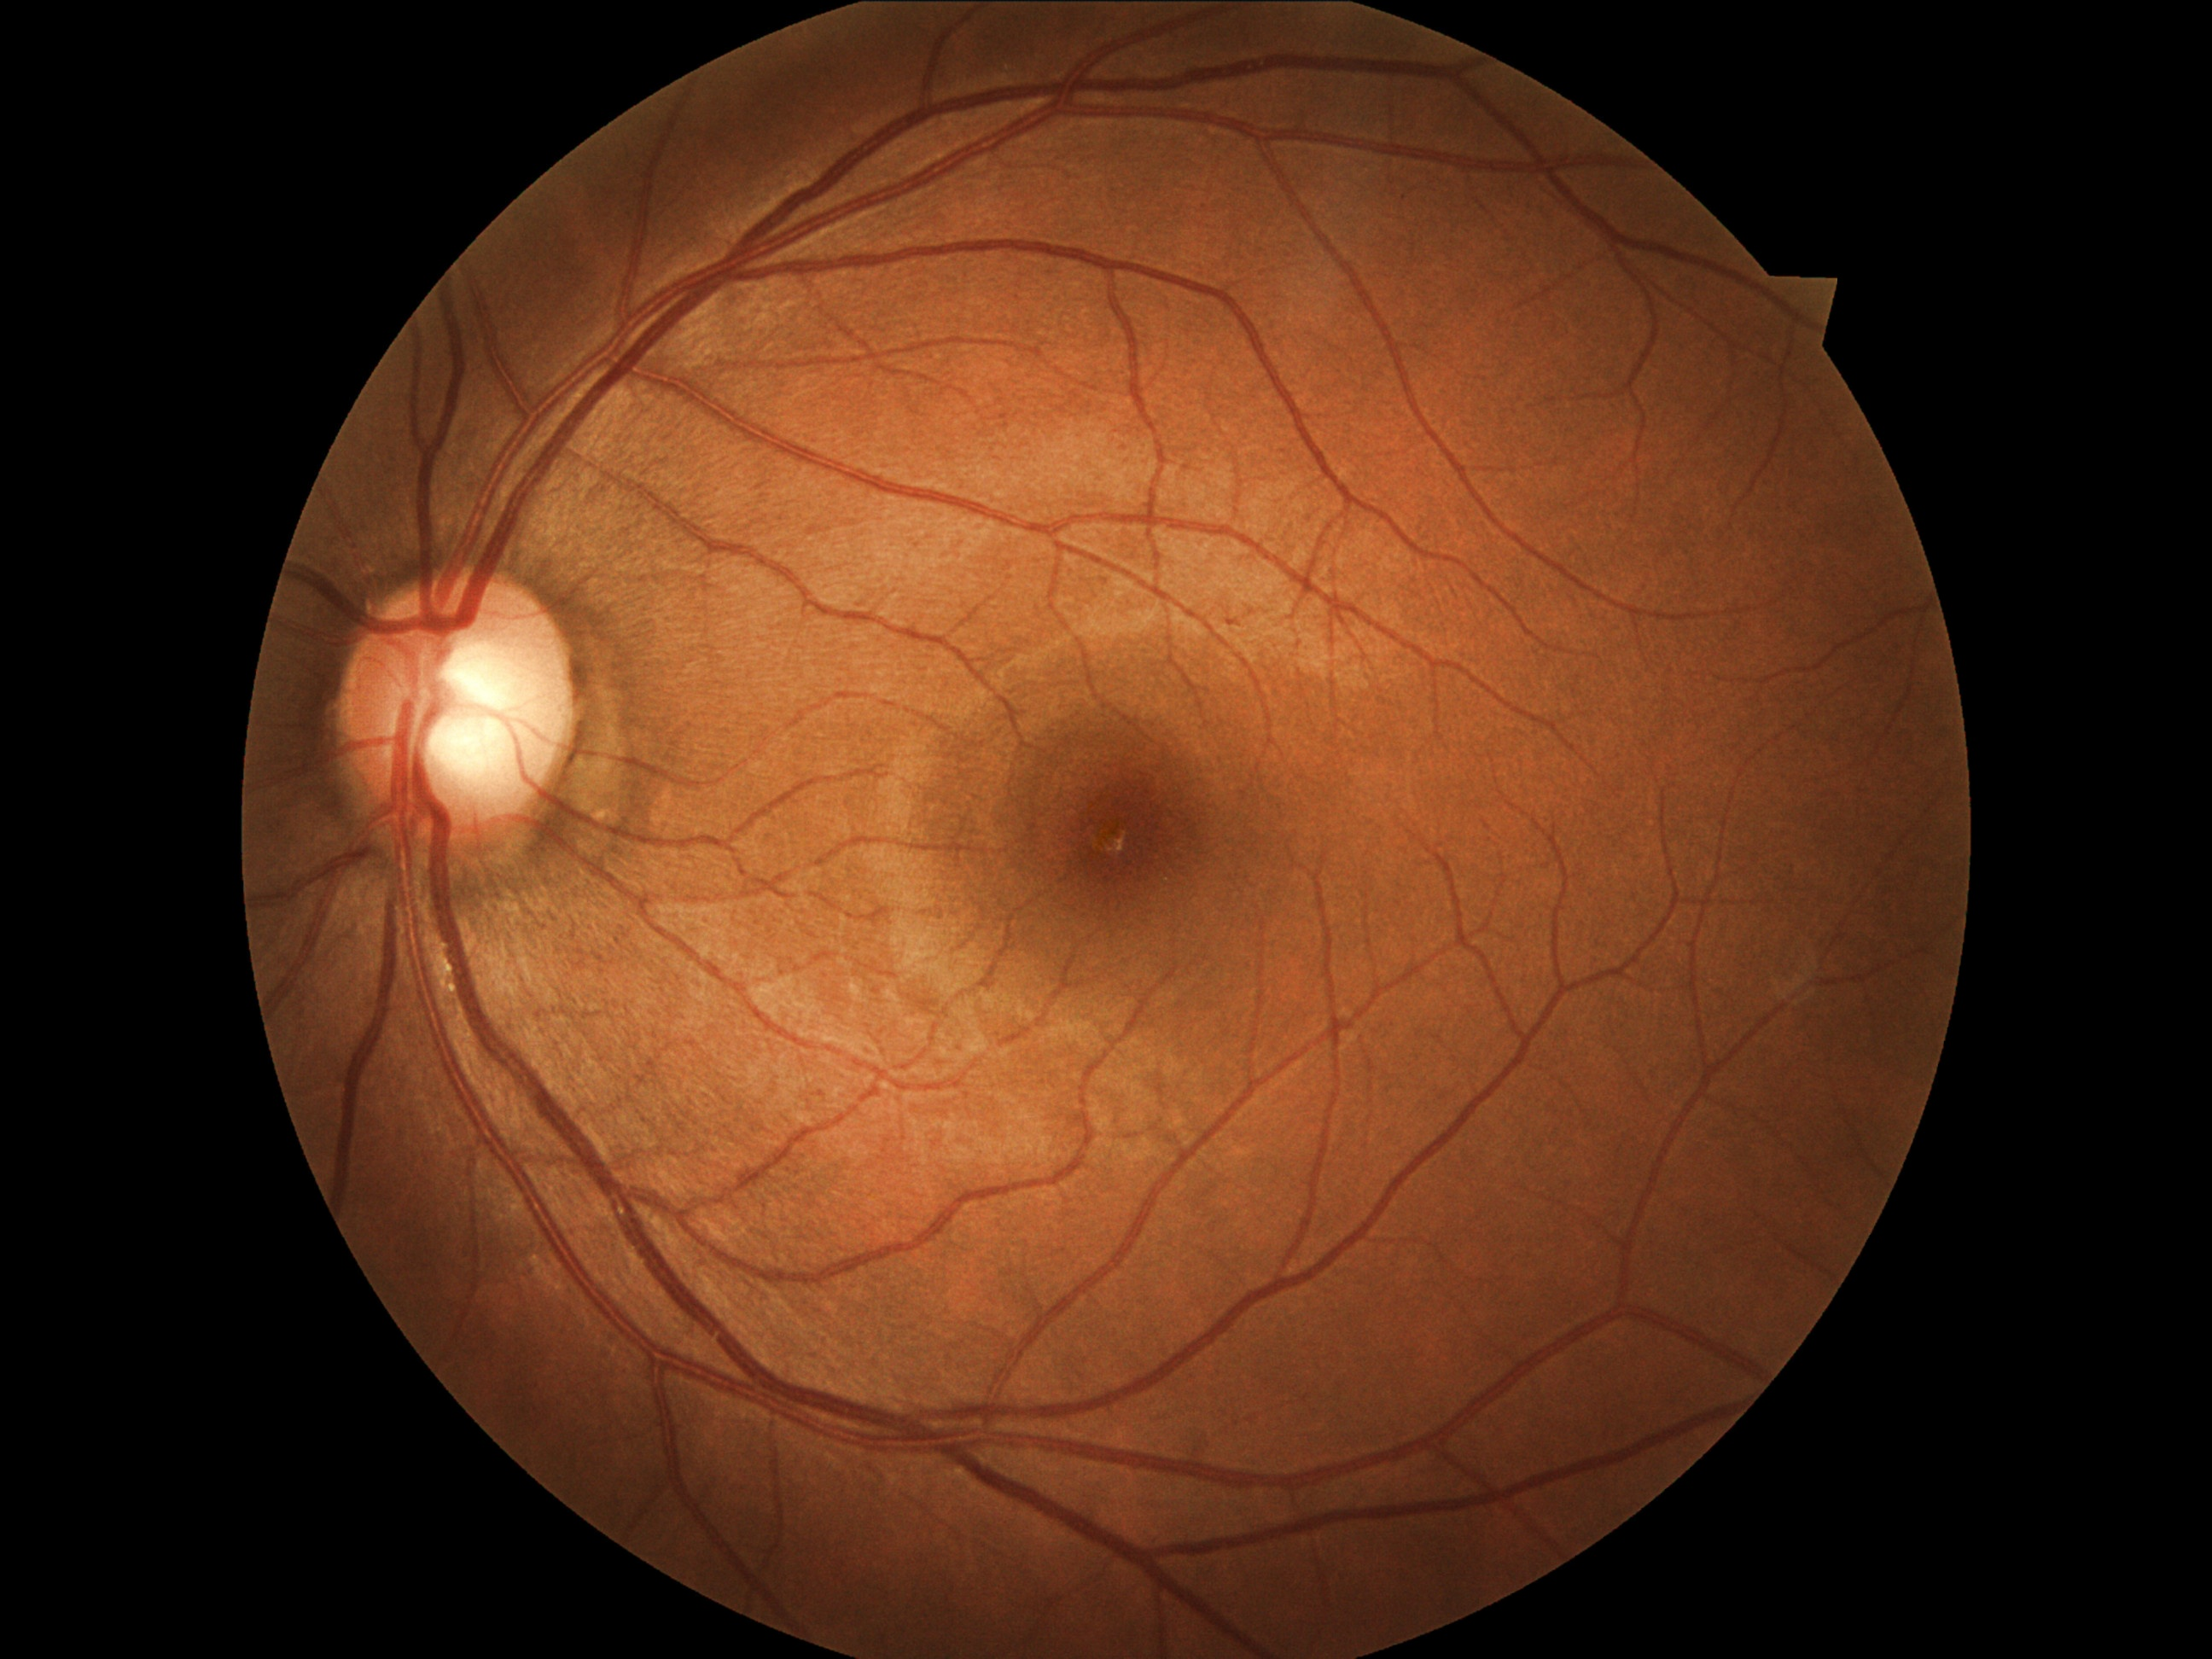
\includegraphics[height=1.3in,width=1.6in]{./images/Color_Histogram/13_left.jpeg}
  }
  \subfigure{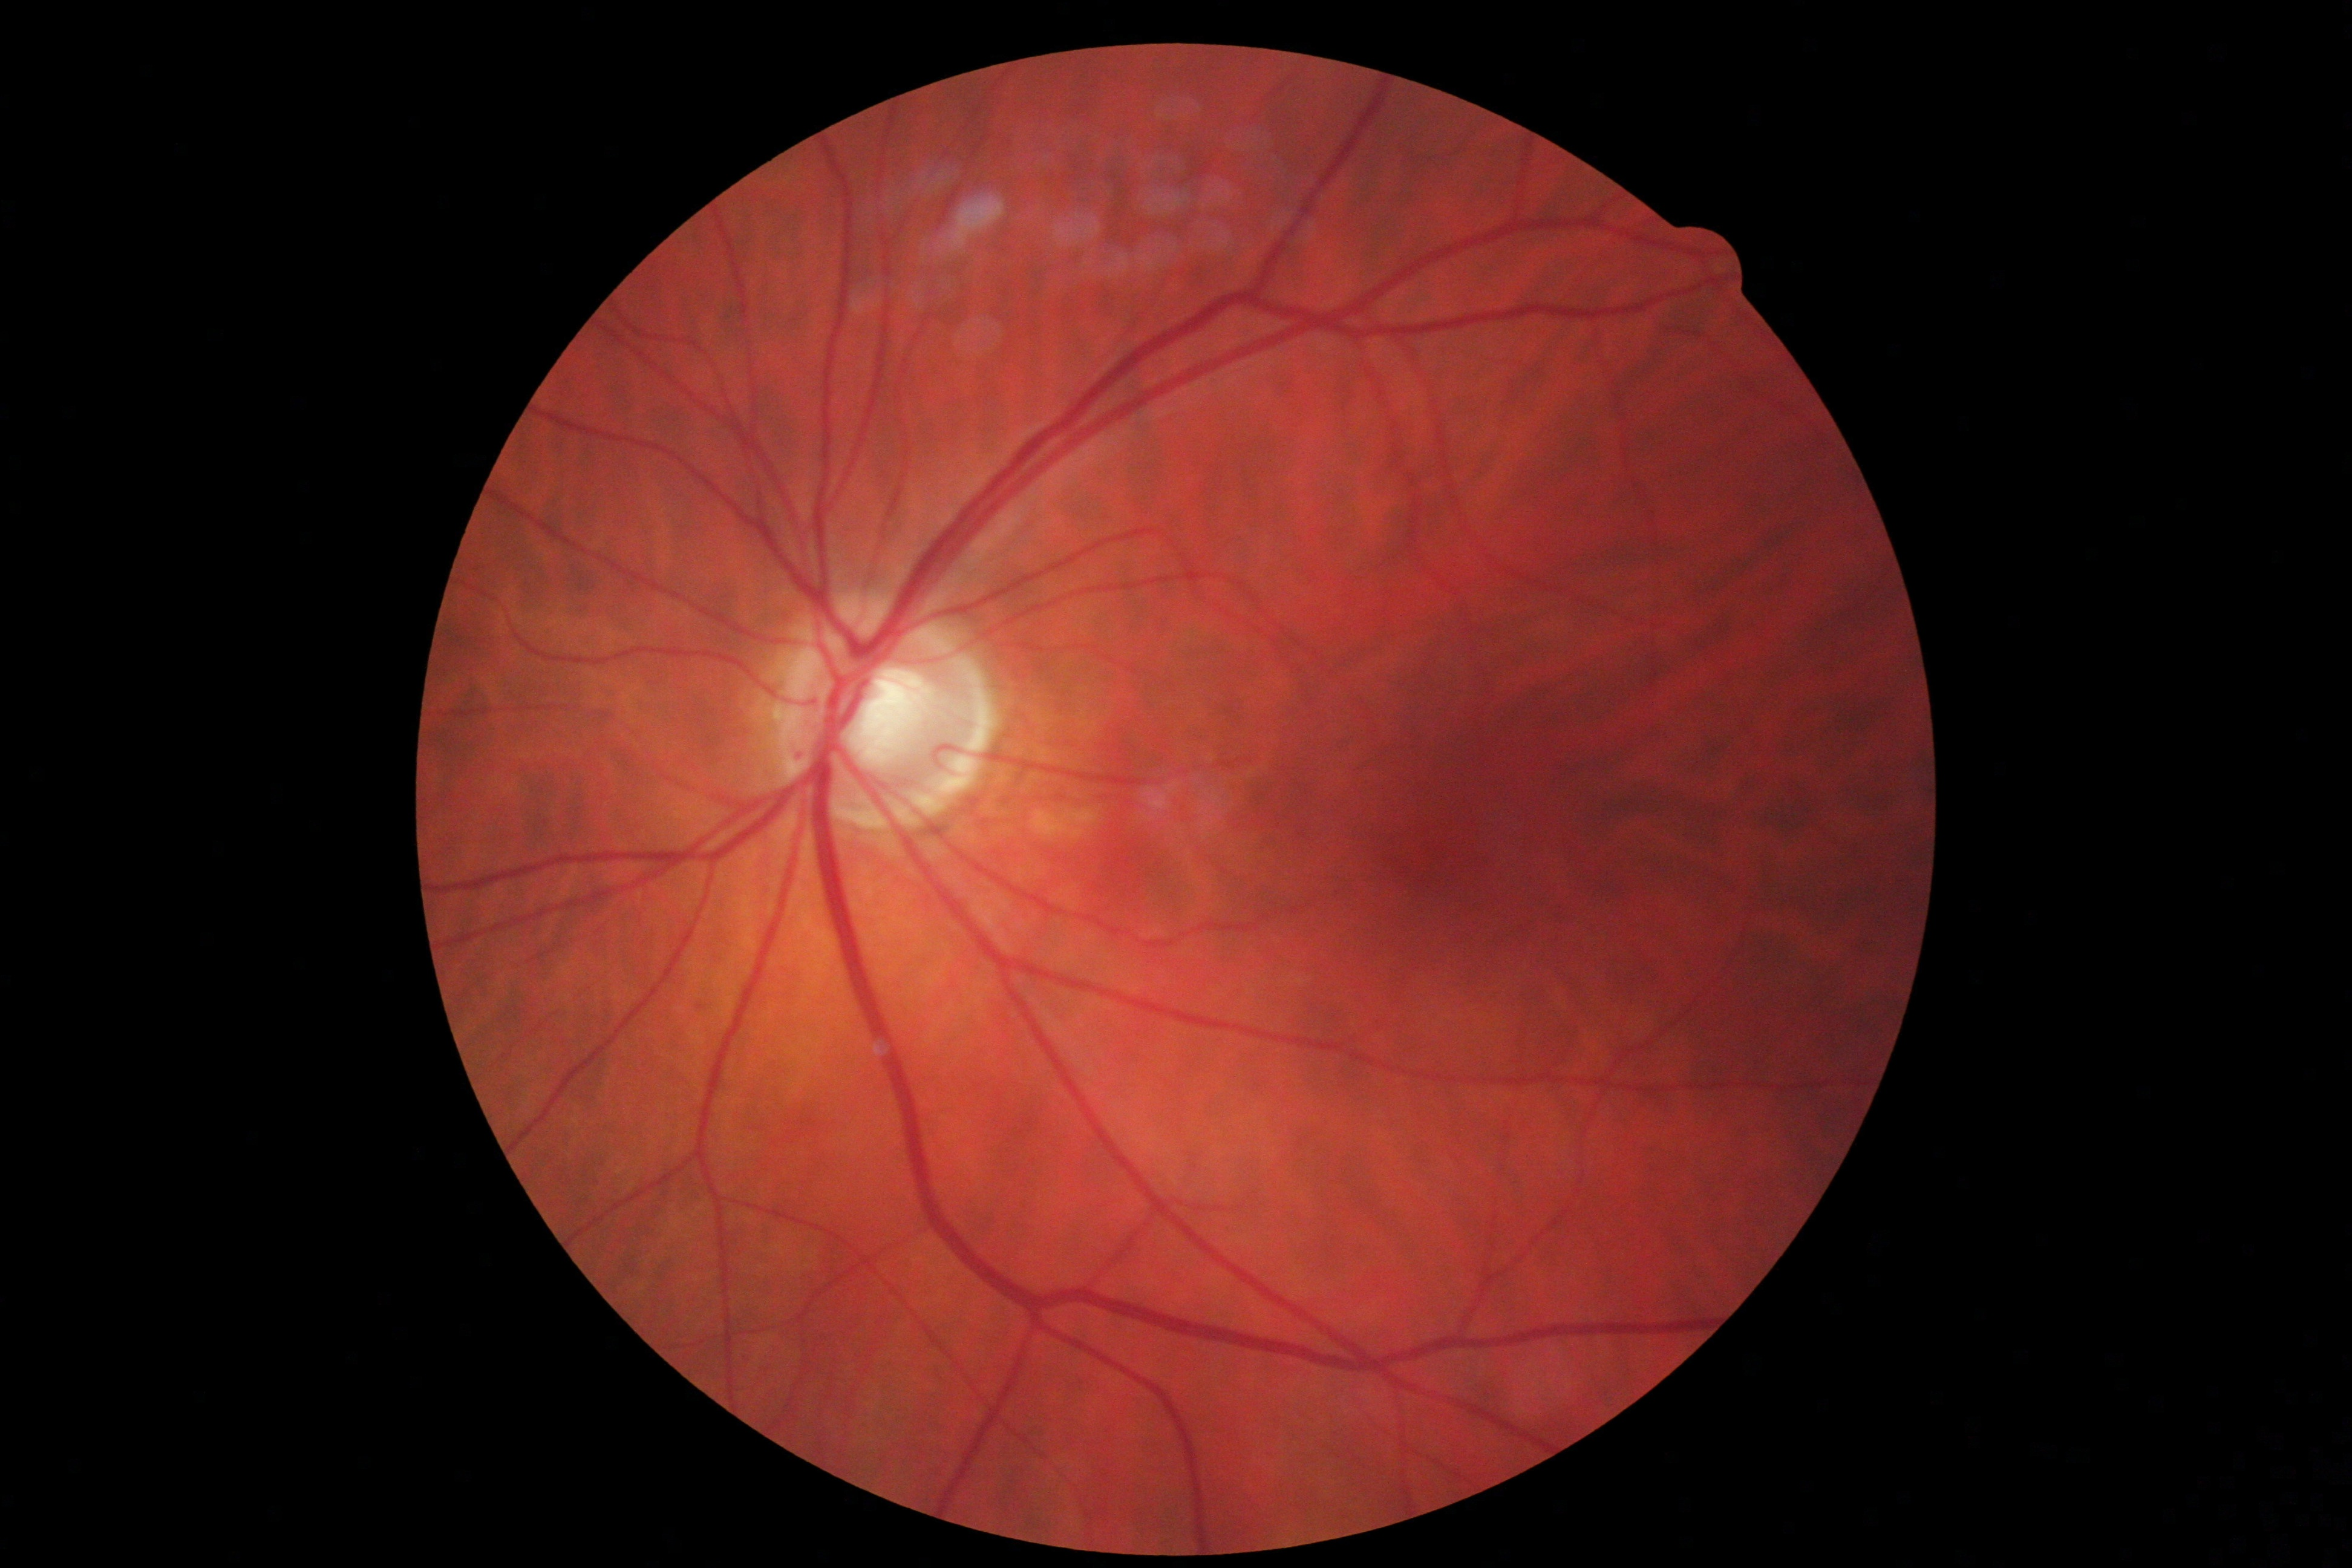
\includegraphics[height=1.3in,width=1.6in]{./images/Color_Histogram/258_left.jpeg}
  }
  \caption{Class 0 images in different lighting conditions}
\end{figure*}

\subsection{Histograms using SIFT Feature Vectors}

Scale-invariant feature transform (SIFT) is a computer vision technique to describe local features and keypoints in images. It is often used in feature tracking and object recognition. We feel that SIFT features can potentially be a useful method of describing eye images and that local eye characteristics will be represented as keypoints in the SIFT feature vectors. For this project, we use $128 \times 1$ dimensional feature vectors.\\ \\
Our method of using SIFT features is as follows. Because we have 35,126 high resolution eye images in total and using all of these images for training is intractable on our local machines, we cut down our dataset to 2,500 images with 500 per class. We first use VLFeat's SIFT library to generate SIFT feature vectors for each image. This process took around 10 hours on our local machines due to the very high resolution of the images. Since the number of SIFT vectors per image is also initially very large, we randomly select $n=20$ SIFT vectors per image. Next, with $n$ SIFT vectors per image, we construct a $128 \times (2,500 \times n)$ SIFT matrix. \\ \\
Our next step is to initialize $K=100$ means from this SIFT matrix. We randomly select $100$ vectors from the SIFT matrix and execute $100$ iterations of the K-means clustering algorithm to converge on a final $128 \times 100$ set of means. \\ \\
Next, for each image, we construct a histogram where each bin is a mean and the frequencies for each mean are the number of times that a SIFT vector for the image is closest to that mean. Thus, every image's histogram has $100$ bins. These histograms are created for both training and testing images.\\ \\
With these histograms we now construct a classifier. We try two different classification methods. Our first method is to use a nearest neighbor search with Euclidean distance. Thus, for a test histogram, we simply find the training histogram that has the shortest Euclidean distance to it and assign it the training image's label. Our second method is to train a multiclass SVM using the training histograms as feature vectors and their respective labels. We found that the multiclass SVM worked significantly better than a nearest-neighbor search using Euclidean distance. \\ \\
The training images we use have both left and right eye orientations. In our evaluation, we decided to train and test exclusively on either left or right images. Using a multiclass SVM, $K=100$, and $n=20$ with 10-fold cross validation our results are: \\ \\
\begin{tabular}{| l | l |}
\hline
Eye side & Average accuracy across 10 folds \\ \hline
Left & 26.15\% \\ \hline
Right & 28.88\% \\ \hline
\end{tabular} \\ \\
Using nearest-neighbor search with the same parameters except $n=40$, our results are: \\ \\
\begin{tabular}{| l | l |}
\hline
Eye side & Average accuracy across 10 folds \\ \hline
Left & 19.65\% \\ \hline
Right & 18.42\% \\ \hline
\end{tabular}  \\ \\
To do futher analysis on why SIFT didn't yield good results, we display SIFT descriptors for each image class. 

\begin{figure*}[htp]
  \centering
  \subfigure[Label 0]{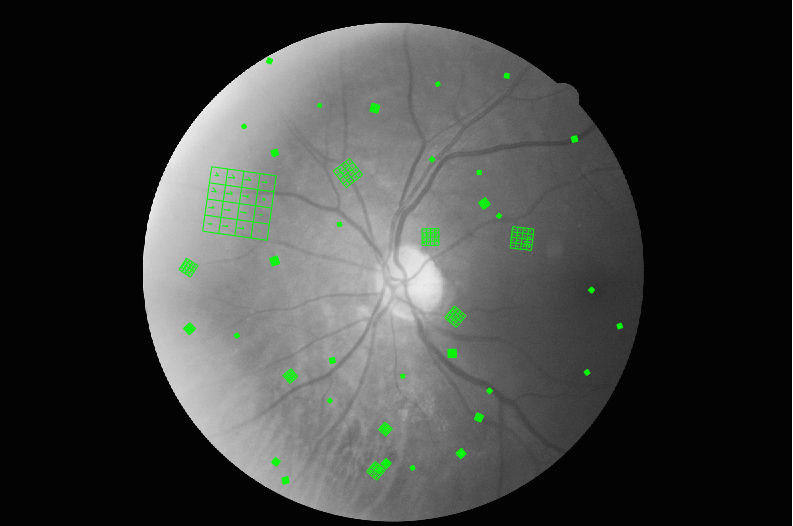
\includegraphics[height=1.3in,width=1.6in]{./images/l0sift.png}
}\quad
  \subfigure[Label 1]{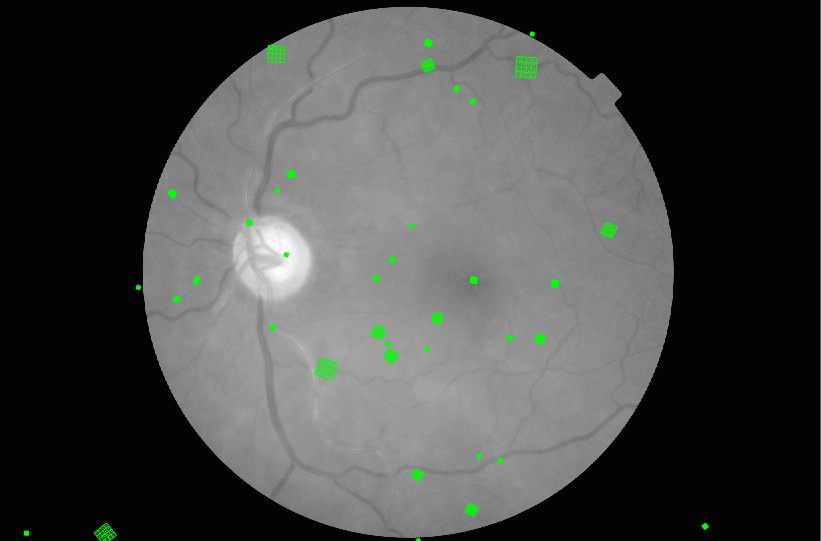
\includegraphics[height=1.3in,width=1.6in]{./images/l1sift.png}
  }\quad
  \subfigure[Label 2]{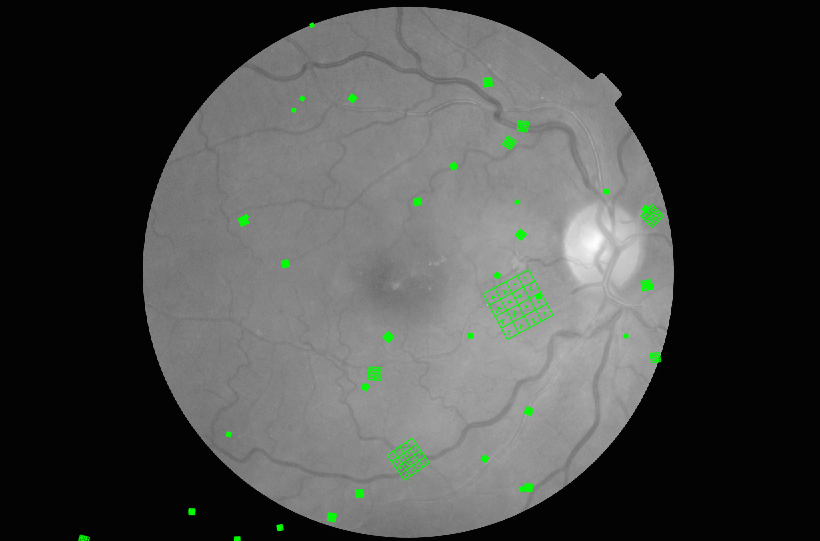
\includegraphics[height=1.3in,width=1.6in]{./images/l2sift.png}
  }\quad
  \subfigure[Label 3]{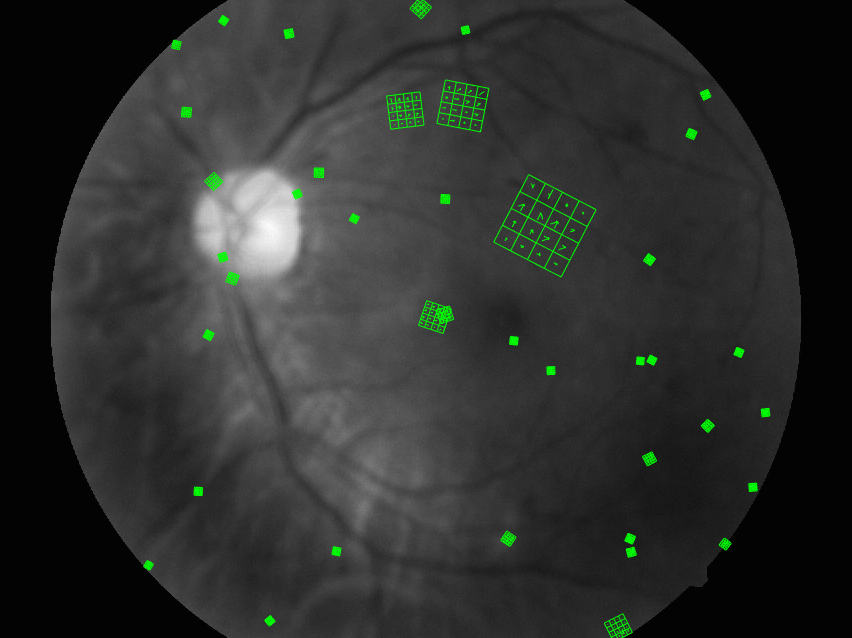
\includegraphics[height=1.3in,width=1.6in]{./images/l3sift.png}
  }\quad
  \subfigure[Label 4]{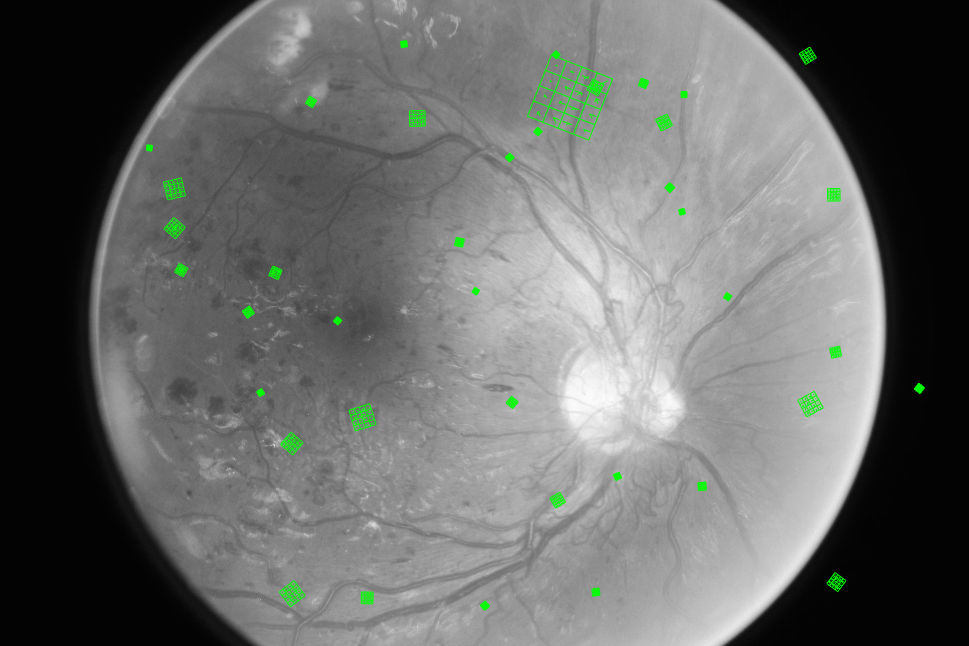
\includegraphics[height=1.3in,width=1.6in]{./images/l4sift.png}
  }\quad
\end{figure*}
The keypoints selected aren't distinctive, often missing exudates and hemorrhages completely. Poor keypoint selection is the primary reason for this method's poor performance. 

\section{Domain-dependent Approaches}
\subsection{Detecting Dot Hemorrhages}
Another result of DR are hemorrhages which are caused by ruptured capillaries and veins. Thus, detecting hemorrhages is useful in determining the severity of DR in a patient image. Below is an example image of dot hemorrhages which was included in Hann's paper.
\begin{figure}[H]
	\centerline{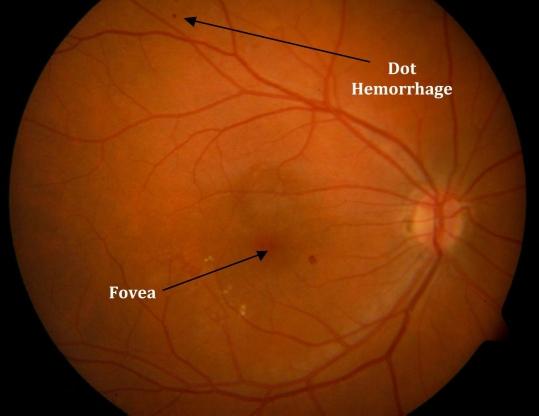
\includegraphics[scale=0.3]{./images/dh.jpg}}
\end{figure}
In the above image, the hemorrhage is a small, dark red dot. We followed the approach of Hann where he first computes the intensity ratios of the red and green channels of each pixel in the image. We then apply horizontal and vertical length 50 median filters to the image which results in two median maps. From each original pixel, we then subtract the minimum value of the maps at the pixel location. Thus, we have \\ \\
$p_{filtered} = p_{original} - min(p_{median_x},p_{median_y})$ \\ \\
Finally, we extract the top 7\% of filtered intensities from $p_{filtered}$. Hann goes on to filter out blood vessels and other non-hemorrhage regions from this filtered intensity map using shape analysis. However, when we performed the initial detection steps using R/G intensities, we found that there was too much noise to be filtered. The images used in Hann's experiment were consistent in color which allowed for hemorrhages to be reliably detected, while minimizing extraneous noise. Our training images exhibit high color variance and oftentimes eye images are bright red which results in too much noise to filter out with shape analysis. We decided not to pursue this feature further, but in the future we hope to use histogram normalization as a solution. Below is an example of our noisy filtered R/G intensity map. Small hemorrhages are detected, but there are also many other circular connected regions.

\begin{figure*}[htp]
  \centering
  \subfigure[Original]{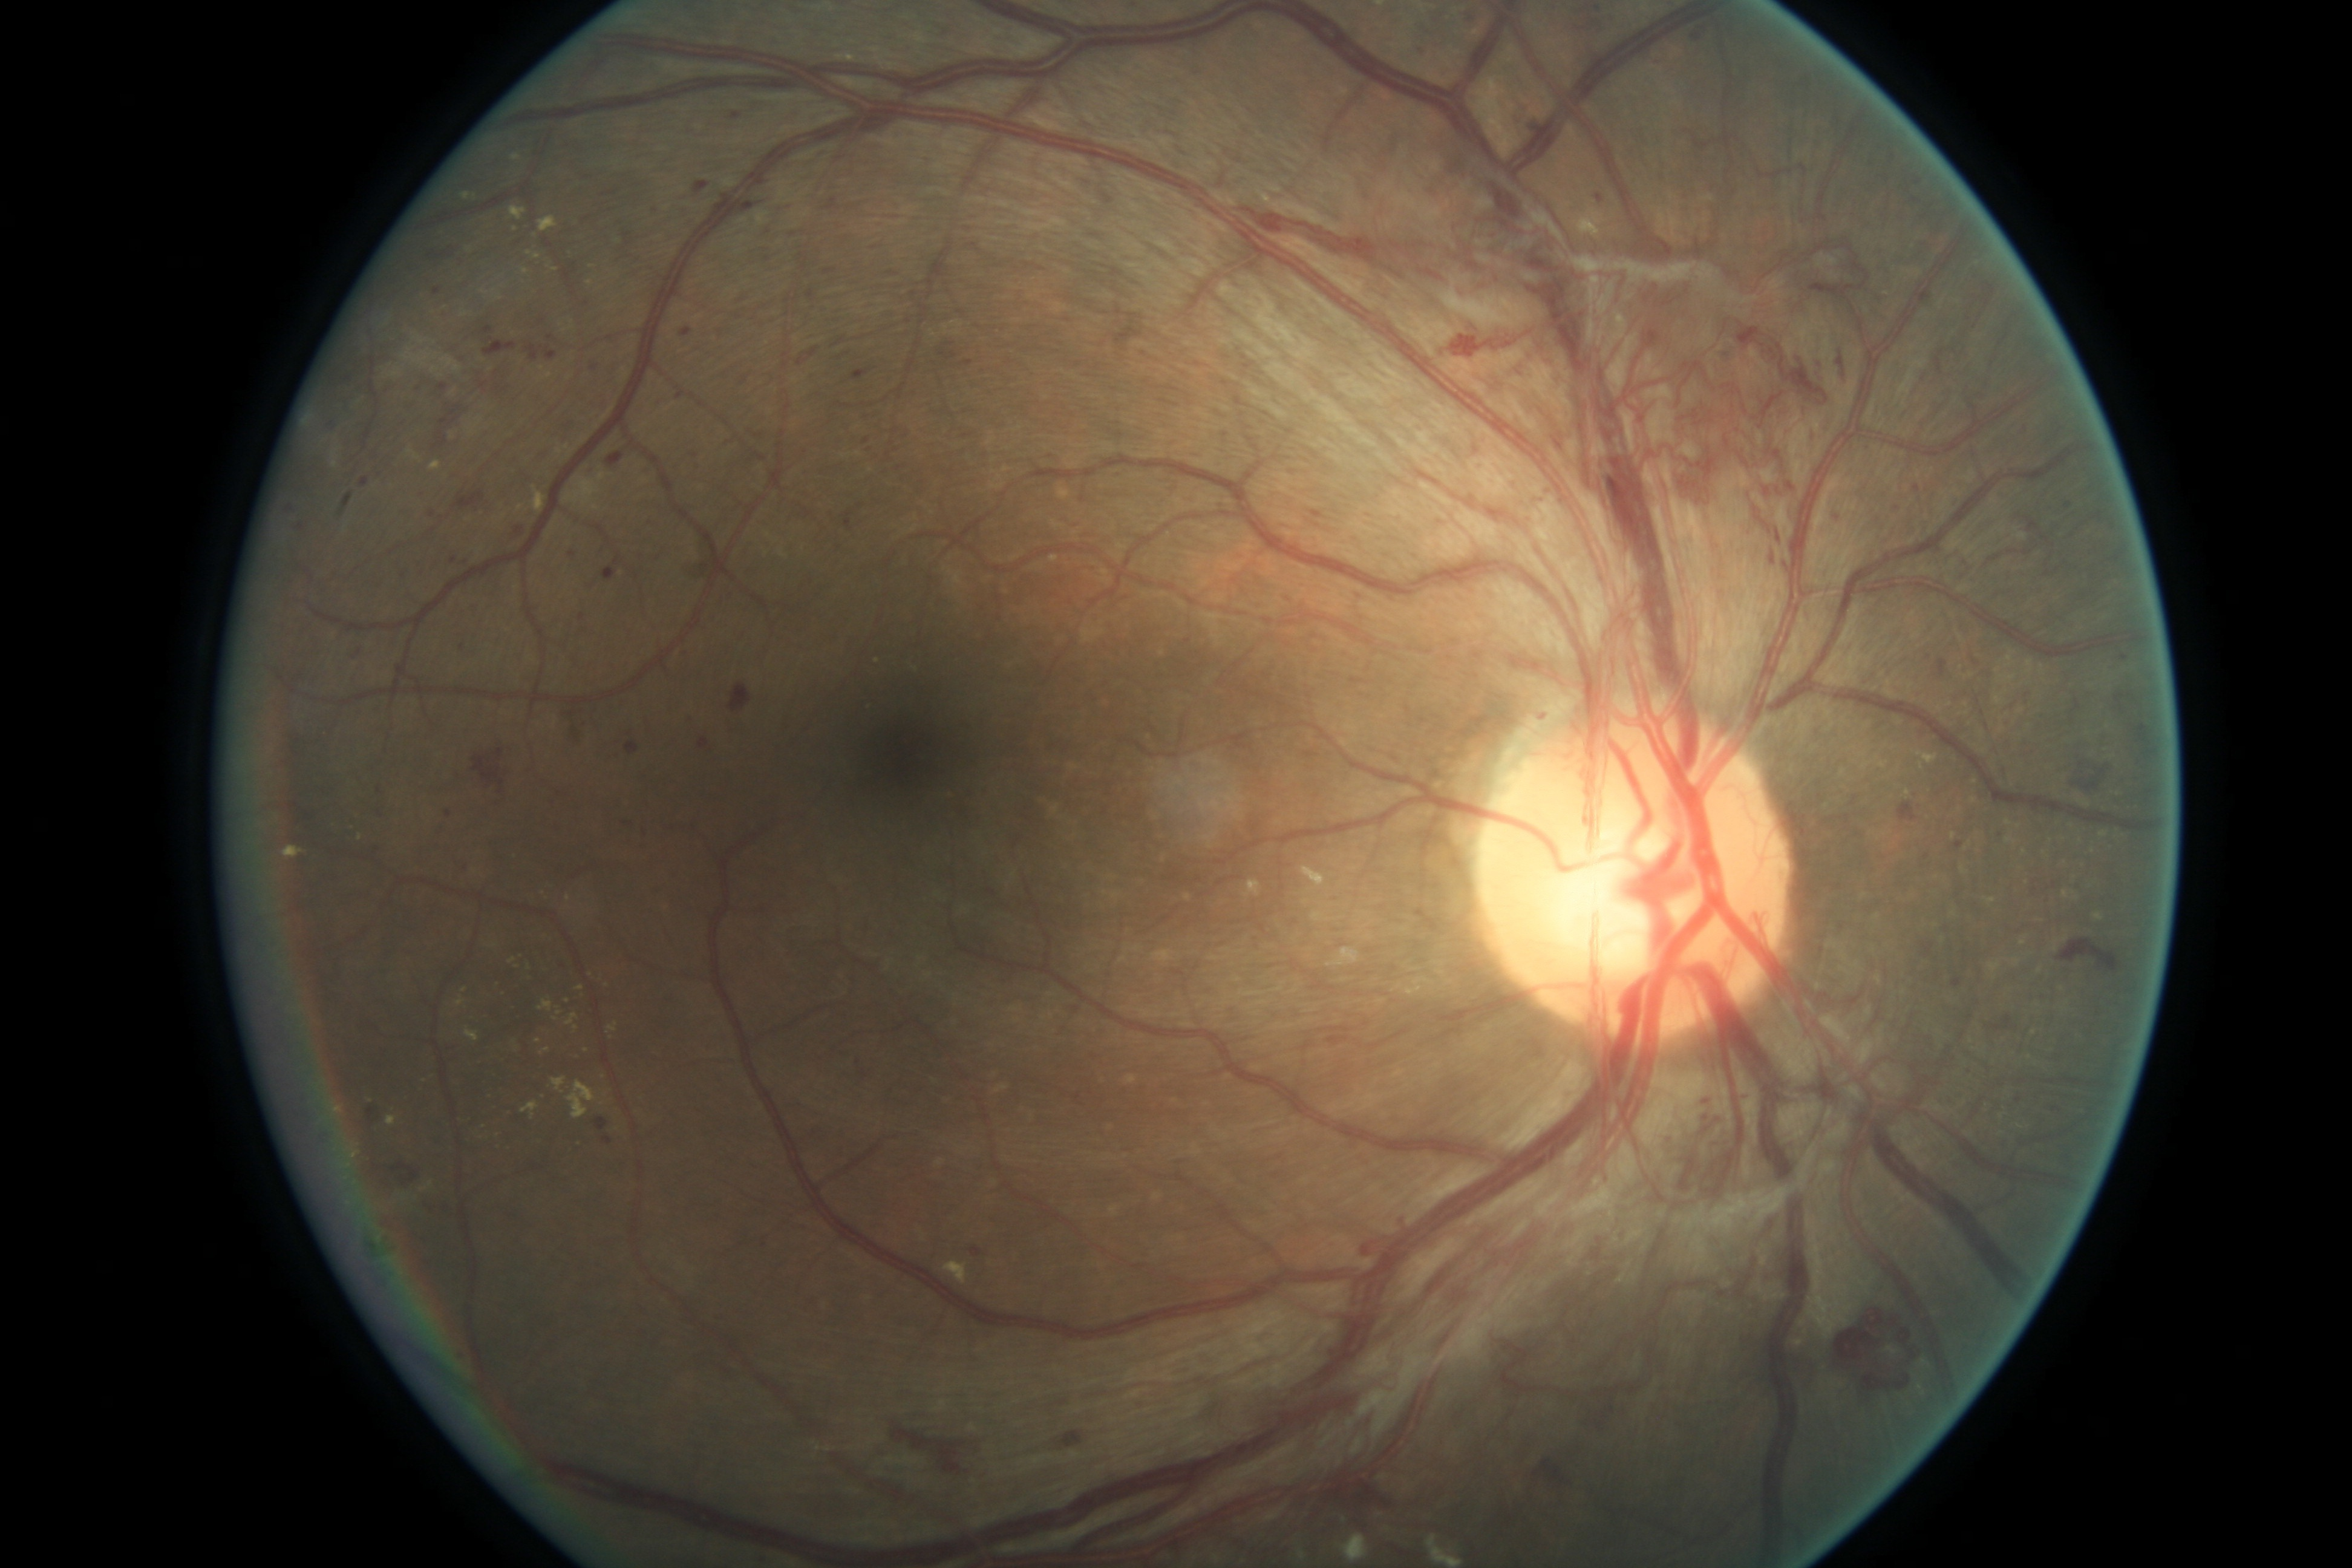
\includegraphics[height=1.3in,width=1.6in]{./images/2804_left.jpeg}
}\quad
  \subfigure[Filtered R/G intensities]{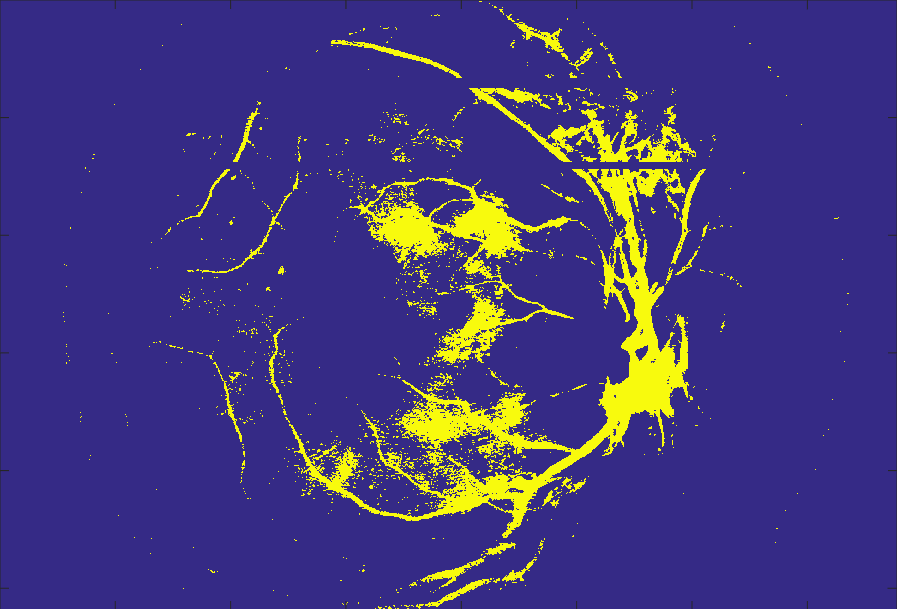
\includegraphics[height=1.3in,width=1.6in]{./images/dh_2804left.png}}
\end{figure*}

\subsection{Detecting Exudates}
Our method of detecting exudates is based on Hann's approach. Exudates often appear as small, bright yellow regions. However, the optic disk is also a bright yellow region. We first identify the optic disk by searching for pixels with large green intensities. More specifically, we obtain the pixels that fall in the top 5\% of green intensities. Our rationale for doing this is because yellow is produced by a combination of large green and red intensities. We then find the largest connected region amongst the selected pixels. Finally, we bound the optic disk with a circle of larger radius and remove all pixels within this circle from consideration when trying to find exudate regions. Below is a visual description of exudates and the optic disk from Hann's paper as well as the results of our optic disc detector.

\begin{figure*}[htp]
  \centering
  \subfigure[Exudate and Optic Disc]{\includegraphics[height=1.5in,width=1.8in]{./images/exudate_odisk.jpg}
}\quad
  \subfigure[Optic Disc detected]{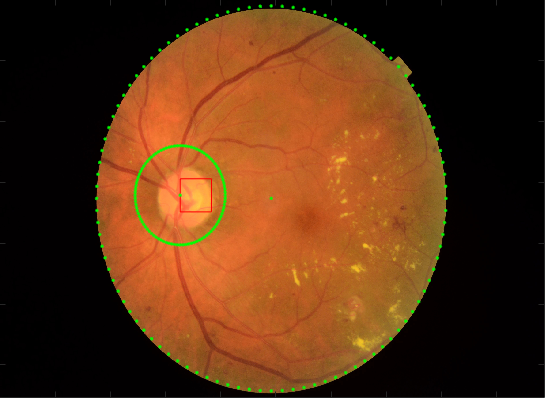
\includegraphics[height=1.5in,width=1.8in]{./images/Exudates_Description/highlight_optic_disc.png}}
\end{figure*}

Realizing that exudate regions correspond to abrupt jumps in color intensities, we apply the aforementioned median filtering methods to obtain a filtered intensity map. We now further examine filtered pixels by selecting those pixels with a filtered value larger than 30. From this new set of pixels, we filter further by selecting those pixels with a green intensity greater than 100. Finally, we filter out pixels that do not belong to a connected component of at least 15 pixels. Below we present the input image and the resultant binary map where exudates are marked white.

\begin{figure*}[htp]
  \centering
  \subfigure[Input Image]{\includegraphics[height=1.5in,width=1.8in]{./images/input_exudate.png}
}\quad
  \subfigure[Output Exudate Map]{\includegraphics[height=1.5in,width=1.8in]{./images/output_exudate.png}
}
\end{figure*}

To classify images, we build a multiclass SVM where the feature for an image is the number of exudate pixels. Using 10-fold cross validation we are able to achieve an accuracy of 30.9\%.

\subsubsection{Light Normalization}
Another challenge we encountered accommodating images with different lighting conditions. We notice that the method described in the paper is very dependent on the color intensities of the image. By observing the example images from the paper, we deduce that the ideal condition for this algorithm is to have bright yellow exudates on a uniform red background. As we mentioned earlier in the color histogram section, our data set contains images with different lighting configurations. We approach this problem by implementing histogram normalization. The process is described below.


\begin{thebibliography}{9}
\bibitem{hann2009}
Hann, C.E. \& Revie, J.A. \& Hewett, D. \& Chase, J.G. \& Shaw, G.M.
(2009) Screening for Diabetic Retinopathy Using Computer Vision and Physiological Markers. 
{\it Journal of Diabetes Science and Technology}
\end{thebibliography}


\end{document}
